\documentclass[openany]{ctexbook}
\usepackage{xeCJK}
\usepackage{amsmath}
\usepackage{titlesec}
\usepackage{booktabs}
\usepackage{tabulary}
\usepackage[multidot]{grffile}
\usepackage{wrapfig}
\usepackage{graphicx}
\usepackage{float}
\usepackage{forest}
\usepackage{tikz}
\usetikzlibrary{matrix}
\usetikzlibrary{arrows}
\usetikzlibrary{positioning}
\usepackage[format=hang,singlelinecheck=0,font={small},labelfont=bf]{subfig}
\usepackage{caption}

\captionsetup[subfigure]{subrefformat=simple,labelformat=simple,listofformat=subsimple}
\renewcommand\thesubfigure{(\alph{subfigure})}

\usepackage{enumitem}
\setlist{nolistsep}
\renewcommand\labelenumi{(\theenumi)}

\usepackage{scrextend}% not needed with a KOMA-Script class, provides the
                      % `addmargin' environment

\usepackage{exsheets}
\DeclareInstance{exsheets-heading}{mylist}{default}{
  runin = true ,
  attach = {
    main[l,vc]number[l,vc](-3.4em,0pt) ; % 3.4em = indent of question body
    main[r,vc]points[l,vc](\linewidth+\marginparsep,0pt)
  }
}
\SetupExSheets{
  headings = mylist , % use the new headings instance
  headings-format = \normalfont\bfseries ,
  counter-within = section ,
  solution/print = true , % print solution or not
  solution/pre-body-hook = {\textsf{答} }
}
\let\oldquestion\question
\let\oldsolution\solution

\renewenvironment{question}{%
	\SetupExSheets{counter-format=\thechapter.qu}
	\oldquestion
}

\renewenvironment{solution}{%
	\SetupExSheets{counter-format=}
	\oldsolution
}

\usepackage{etoolbox}
% 3em = indent of question body :
\AtBeginEnvironment{question}{\addmargin[3em]{0em}}
\AtEndEnvironment{question}{\endaddmargin}
\AtBeginEnvironment{solution}{\addmargin[3em]{0em}}
\AtEndEnvironment{solution}{\endaddmargin}

\title{人工智能及其应用(第4版)\\ 习题解析}
\date{}

\begin{document}
\maketitle

\setlength{\abovedisplayskip}{3pt}
\setlength{\belowdisplayskip}{3pt}

\chapter{绪论}

\begin{question}
什么是人工智能?试从学科和能力两方面加以说明。
\end{question}	
\begin{solution}
人工智能(学科):人工智能(学科)是计算机科学中涉及研究、设计和应用智能机器的一个分支。其近期主要目标在于研究用机器来模仿和执行人脑的某些智力功能,并开发相关理论和技术。\par
人工智能(能力):人工智能(能力)是智能机器所执行的通常与人类智能有关的智能行为,这些智能行为涉及学习、感知、思考、理解、识别、判断、推理、证明、通信、设计、规划、行动和问题求解等活动。
\end{solution}

\begin{question}
在人工智能的发展过程中,有哪些思想和思潮起了重要作用?
\end{question}
\begin{solution}
控制论之父维纳1940年主张计算机五原则。他开始考虑计算机如何能像大脑一样工作。系统地创建了控制论,根据这一理论,一个机械系统完全能进行运算和记忆。\par
帕梅拉·麦考达克(Pamela McCorduck)在她的著名的人工智能历史研究《机器思维》(\textit{Machine Who Think}, 1979)中曾经指出:在复杂的机械装置与智能之间存在着长期的联系。\par
著名的英国科学家图灵被称为人工智能之父,图灵不仅创造了一个简单的通用的非数字计算模型,而且直接证明了计算机可能以某种被理解为智能的方法工作。提出了著名的图灵测试。\par
数理逻辑从19世纪末起就获迅速发展;到20世纪30年代开始用于描述智能行为。计算机出现后,又在计算机上实现了逻辑演绎系统。\par
1943年由生理学家麦卡洛克(McCulloch)和数理逻辑学家皮茨(Pitts)创立的脑模型,即MP模型。60-70年代,联结主义,尤其是对以感知机(perceptron)为代表的脑模型的研究曾出现过热潮。\par
控制论思想早在40-50年代就成为时代思潮的重要部分,影响了早期的人工智能工作者。到60-70年代,控制论系统的研究取得一定进展,播下智能控制和智能机器人的种子。 
\end{solution}

\begin{question}
在过去的20年中,人工智能发生了什么变化?
\end{question}
\begin{solution}
\end{solution}

\begin{question}
为什么能够用机器(计算机)模仿人的智能?
\end{question}
\begin{solution}
物理符号系统假设:任何一个系统,如果它能够表现出智能,那么它就必定能够执行输入符号、输出符号、存储符号、复制符号、建立符号结构、条件性迁移6种功能。反之,任何系统如果具有这6种功能,那么它就能够表现出智能;这种智能指的是人类所具有的那种智能。\par
物理符号系统的假设伴随有3个推论:\par
	\begin{enumerate}
		\item 既然人具有智能,那么他(她)就一定是个物理符号系统。
		\item 既然计算机是一个物理符号系统,它就一定能够表现出智能。
		\item 既然人是一个物理符号系统,计算机也是一个物理符号系统,那么我们就能够用计算机来模拟人的活动。
	\end{enumerate} \par
因此,计算机可以模拟人的智能。
\end{solution}

\begin{question}
现在人工智能有哪些学派?它们的认知观是什么?现在这些学派的关系如何?
\end{question}
\begin{solution}
符号主义(Symbolicism),又称为逻辑主义(Logicism)、心理学派(Psychlogism)或计算机学派(Computerism),认为人工智能源于数理逻辑。 其原理主要为物理符号系统(即符号操作系统)假设和有限合理性原理。符号主义认为人的认知基元是符号,而且认知过程即符号操作过程。它认为人是一个物理符号系统,计算机也是一个物理符号系统,因此,我们就能够用计算机来模拟人的智能行为。它还认为,知识是信息的一种形式,是构成智能的基础。人工智能的核心问题是知识表示、知识推理和知识运用。 符号主义认为人工智能的研究方法应为功能模拟方法。通过分析人类认知系统所具备的功能和技能,然后用计算机模拟这些功能,实现人工智能。\par
连接主义(Connectionism),又称为仿生学派(Bionicsism)或生理学派(Physiologism) ,认为人工智能源于仿生学,特别是人脑模型的研究。其原理主要为神经网络及神经网络间的连接机制与学习算法。连接主义认为人的思维基元是神经元,而不是符号处理过程。认为人脑不同于电脑,并提出联结主义的大脑工作模式,用于取代符号操作的电脑工作模式。 连接主义主张人工智能应着重于结构模拟,即模拟人的胜利神经网络结构,并认为功能、结构和智能行为是密切相关的。不同的结构表现出不同的功能和行为。\par
行为主义(Actionism),又称进化主义(Evolutionism)或控制论学派(Cyberneticsism), 认为人工智能源于控制论。其原理为控制论及感知-动作型控制系统 。行为主义认为智能取决于感知和行动,提出智能行为的“感知-动作”模式。认为智能不需要知识、不需要表示、不需要推理;人工智能可以像人类智能一样逐步进化。智能行为只能在现实世界中与周围环境交互作用而表现出来。行为主义还认为:符号主义、联结主义对真实世界客观事物的描述及其智能行为工作模式是过于简化的抽象,因而是不能真实地反映客观存在的。 行为主义认为人工智能的研究方法应采用行为模拟方法,也认为功能、结构和智能行为是不可分的。不同行为表现出不同功能和不同控制结构。
\end{solution}

\begin{question}
你认为应从哪些层次对认知行为进行研究?
\end{question}
\begin{solution}
人的认知活动具有不同的层次,对认知行为的研究也应具有不同的层次,以便不同学科之间分工协作,联合攻关,早日解开人类认知本质之谜。可以从下列4个层次开展对认知本质的研究: 
	\begin{enumerate}
		\item 认知生理学:研究认知行为的生理过程,主要研究人的神经系统(神经元、中枢 神经系统和大脑)的活动,是认知科学研究的底层。它与心理学、神经学、脑科学有密切关系,且与基因学、遗传学等有交叉联系。
		\item 认知心理学:研究认知行为的心理活动,主要研究人的思维策略,是认知科学研究的顶层。它与心理学有密切关系,且与人类学、语言学交叉。
		\item 认知信息学:研究人的认知行为在人体内的初级信息处理,主要研究人的认知行为如何通过初级信息自然处理,由生理活动变为心理活动及其逆过程,即由心理活动变为生理行为。这是认知活动的中间层,承上启下。它与神经学、信息学、计算机科学有模切关系,并与心理学、生理学有交叉。
		\item 认知工程学:研究认知行为的信息加工处理,主要研究如何通过以计算机为中心的人工信息处理系统,对人的各种认知行为(如知觉、思维、记忆、语言、学习、理解、推理、识别等)进行信息处理。 这是研究认知科学和认知行为的工具,应成为现代认知心理学和现代认知生理学的重要研究手段。它与人工智能、信息学、计算机科学有密切关系,并与控制论、系统学等交叉。
	\end{enumerate} \par
心理活动的最高层级是思维策略,中间一层是初级信息处理,最低层级是生理过程,与此相应的是计算机程序、语言和硬件。 研究认知过程的主要任务是探求高层次思维决策与初级信息处理的关系,并用计算机程序来模拟人的思维策略水平,而用计算机语言模拟人的初级信息处理过程。 
\end{solution}

\begin{question}
你是如何理解人工智能的研究目标的?
\end{question}
\begin{solution}
\end{solution}

\begin{question}
人工智能研究包括哪些内容?这些内容的重要性如何?
\end{question}
\begin{solution}
分布式人工智能、知识工程和专家系统、自然语言处理、机器学习、机器人、模式识别、自动定理证明、自动程序设计、智能数据库、智能检索等。
\end{solution}

\begin{question}
人工智能的基本研究方法有哪几类?它们与人工智能学派的关系如何?
\end{question}
\begin{solution}
\end{solution}

\begin{question}
人工智能的主要研究和应用领域是什么?其中,哪些是新的研究热点?
\end{question}
\begin{solution}
人工智能的主要研究和应用领域有:问题求解与博弈(下棋程序),逻辑推理与定理证明(四色定理证明),计算智能,分布式人工智能与Agent,自动程序设计,专家系统,机器学习,自然语言理解,机器人学(星际探索机器人),模式识别(手写识别,汽车牌照识别,指纹识别),机器视觉(机器装配,卫星图像处理),神经网络,智能控制,智能调度与指挥(汽车运输高度,列车编组指挥),智能检索,系统与语言工具等。 \par
其中新的研究热点有:分布式人工智能与Agent,计算智能与进化计算,数据挖掘与知识发现,人工生命。
\end{solution}

\begin{question}
你对人工智能课程教学有何意见和建议?
\end{question}
\begin{solution}
\end{solution}
\chapter{知识表示方法}

\begin{question}
状态空间法、问题归约法、谓词逻辑法和语义网络法的要点是什么?它们有何本质上的联系及异同点?
\end{question}	
\begin{solution}
状态空间法:基于解答空间的问题表示和求解方法,它是以状态和算符为基础来表示和求解问题的。一般用状态空间法来表示下述方法:从某个初始状态开始,每次加一个操作符,递增的建立起操作符的试验序列,直到达到目标状态为止。 \par
问题规约法:已知问题的描述,通过一系列变换把此问题最终变成一个子问题集合:这些子问题的解可以直接得到,从而解决了初始问题。问题规约的实质:从目标(要解决的问题)出发逆向推理,建立子问题以及子问题的子问题,直至最后把出示问题规约为一个平凡的本原问题集合。 \par
谓词逻辑法:采用谓词合式公式和一阶谓词算法。要解决的问题变为一个有待证明的问题,然后采用消解定理和消解反演莱证明一个新语句是从已知的正确语句导出的,从而证明这个新语句也是正确的。\par
语义网络法:是一种结构化表示方法,它由节点和弧线或链组成。节点用于表示物体、概念和状态,弧线用于表示节点间的关系。语义网络的解答是一个经过推理和匹配而得到的具有明确结果的新的语义网络。语义网络可用于表示多元关系,扩展后可以表示更复杂的问题。
\end{solution}

\begin{question}
设有$3$个传教士和$3$个野人来到河边,打算成一条船从右岸渡到左岸去。该船的负载能力为两人。在任何时候,如果野人人数超过传教士人数,那么野人就会把传教士吃掉。怎样才能用这条船安全地把所有人都渡过河去?
\end{question}
\begin{solution}
设$(m,n)$表示右岸上有$m$个野人,$n$个传教士;$r(m,n)$表示把$m$个野人和$n$个传教士从右岸运至左岸,$l(m,n)$表示把$m$个野人和$n$个传教士从左岸运至右岸。则安全把所有人渡过河的过程表示为
\begin{align*}
& (3,3) \xrightarrow{r(2,0)} (1,3) \xrightarrow{l(1,0)} (2,3) 
	\xrightarrow{r(2,0)} (0,3) \xrightarrow{l(1,0)} (1,3) \\
	\xrightarrow{r(0,2)} & (1,1) \xrightarrow{l(1,1)} (2,2) 
	\xrightarrow{r(0,2)} (2,0) \xrightarrow{l(1,0)} (0,0) \xrightarrow{r(2,0)} (0,0)
\end{align*}
\end{solution}

\begin{question}
利用图\ref{Fig:TSP-problem},用状态空间法规划一个最短的旅行路程:此旅程从城市A开始,访问其他城市不多于一次,并返回A。选择一个状态表示,表示出所求得的状态空间的节点及弧线,标出适当的代价,并指明图中从起始节点到目标节点的最佳路径。
\end{question}
\begin{solution}
用状态空间法表示所求路径如图\ref{Fig:TSP-answer}所示。
	\begin{figure} [h]
		\centering
	\end{figure}
\end{solution}

\begin{question}
试说明怎样用一棵与或解树来表达图\ref{Fig:elec}所示的电网络阻抗的计算。单独的$R$、$L$或$C$可分别用$R$、$j\omega L$或$1/j\omega C$来计算,这个事实用作本原问题。后继算符应以复合并联和串联阻抗的规则为基础。
\end{question}
\begin{solution}
约定,用原来的与后继算法用来表达并联关系,用原来的或后继算法用来表达串联关系。则所求与或解树如图\ref{Fig:and-or-tree-for-elec}所示。
\end{solution}

\begin{question}
试用四元数列结构表示四圆盘梵塔问题,并画出求解该问题的与或图。
\end{question}
\begin{solution}
用四元数列$(n_A, n_B, n_C, n_D)$来表示A、B、C、D盘分别落在$n_A$、$n_B$、$n_C$、$n_D$号柱子上。则问题科的初始状态为$(1,1,1,1)$,目标状态为$(3,3,3,3)$。\par
求解问题的与或图如图\ref{Fig:and-or-tree-for-hannoi},按从上往下的顺序,依次处理每一个叶结点,搬动圆盘,问题得解。 
\end{solution}

	\begin{figure}[H]
		\centering
		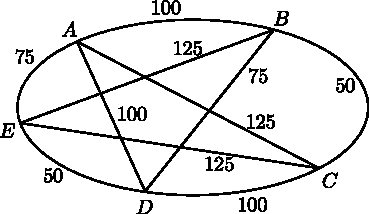
\includegraphics[scale=.8]{figures/ques-2.3.pdf}
		\caption{旅行商问题} \label{Fig:TSP-problem}
		\vspace{1cm}
				\begin{forest}
		  for tree={
		    draw,
		    circle,
		  },
		  [A
		  	[B, edge label={node[midway,left,font=\scriptsize]{100}}
		  		[C, edge label={node[midway,left,font=\scriptsize]{150}}
		  			[D, edge label={node[midway,left,font=\scriptsize]{100}}
		  				[E, edge label={node[midway,right,font=\scriptsize]{50}}
		  					[A, edge label={node[midway,right,font=\scriptsize]{75}}
		  					]]]
		  			[E, edge label={node[midway,right,font=\scriptsize]{125}}
		  				[D, edge label={node[midway,right,font=\scriptsize]{50}}
		  					[A, edge label={node[midway,right,font=\scriptsize]{100}}
		  					]]]
		  		][D, edge label={node[midway,right,font=\scriptsize]{75	}}
		  			[C, edge label={node[midway,left,font=\scriptsize]{100}}
		  				[E, edge label={node[midway,right,font=\scriptsize]{125}}
		  					[A, edge label={node[midway,right,font=\scriptsize]{75}}
		  					]]]
		  			[E, edge label={node[midway,right,font=\scriptsize]{50}}
		  				[C, edge label={node[midway,right,font=\scriptsize]{125}}
		  					[A, edge label={node[midway,right,font=\scriptsize]{125}}
		  					]]]
		  		][E, edge label={node[midway,right,font=\scriptsize]{125}}
					[C, edge label={node[midway,left,font=\scriptsize]{125}}
						[D, edge label={node[midway,right,font=\scriptsize]{100}}
							[A, edge label={node[midway,right,font=\scriptsize]{100}}
							]]]
					[D, edge label={node[midway,right,font=\scriptsize]{50}}
						[C, edge label={node[midway,right,font=\scriptsize]{100}}
							[A, edge label={node[midway,right,font=\scriptsize]{125}}
							]]]  		
		  		]
		  	][C][D][E]
		  ]
		\end{forest}
		\caption{旅行商问题状态空间图} \label{Fig:TSP-answer}
		\vspace{1cm}
		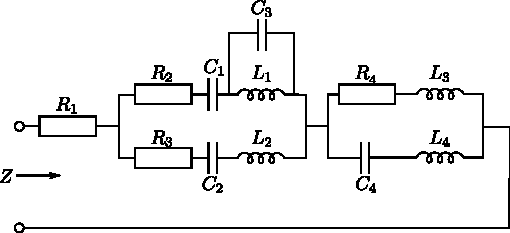
\includegraphics{figures/ques-2.4.pdf}
		\caption{电网络阻抗计算} \label{Fig:elec}
	\end{figure}
	
	\begin{figure}[H]
		\centering
		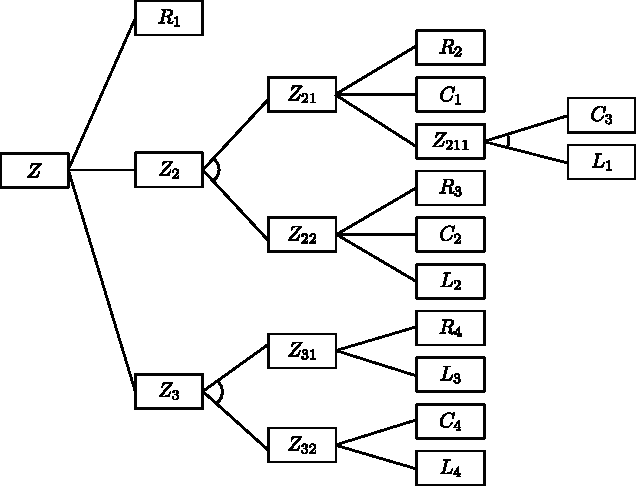
\includegraphics[scale=.8]{figures/ans-2.4.pdf}
		\caption{电网络阻抗计算与或解树} \label{Fig:and-or-tree-for-elec}
		\vspace{1cm}
		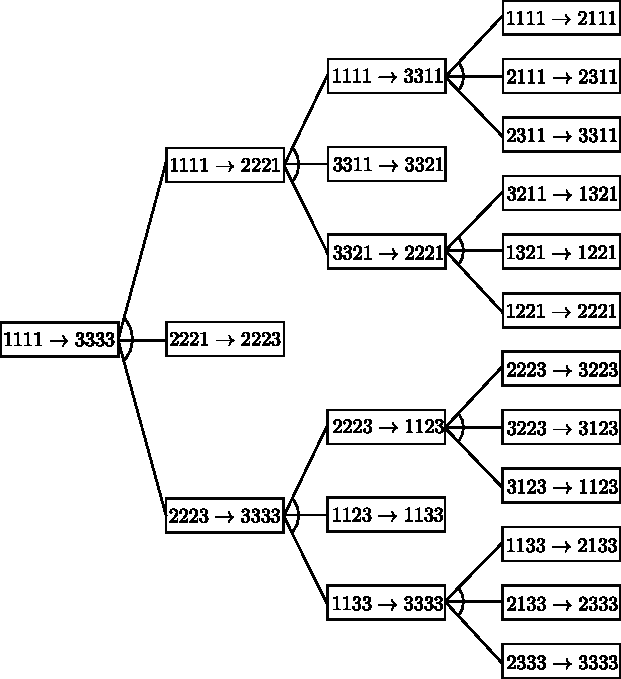
\includegraphics[scale=.8]{figures/ans-2.5.pdf}
		\caption{樊塔问题与或树} \label{Fig:and-or-tree-for-hannoi}
	\end{figure}

\begin{question}
把下列句子变换成子句形式:
	\begin{enumerate}
         \item $\left(\forall x\right) \left\{P\left(x\right) \to P\left(x\right)\right\}$
         \item $\forall x \forall y \left(\mathrm{On} \left(x,y\right) \to \mathrm{Above} \left(x,y\right) \right)$
         \item $\forall x \forall y \forall z \left(\mathrm{Above} \left(x,y\right) \wedge \mathrm{Above}\left(y,z\right) \to \mathrm{Above}\left(x,z\right) \right)$ 
         \item $\sim\left\{\left(\forall x\right)\left\{\left(\forall y)\left[p\left(y\right) \to p(f(x,y))\right] \wedge \left(\forall y \right) \left[Q(x,y) \to P(y) \right]\right\}\right\}\right\}$
	\end{enumerate}
\end{question}
\begin{solution}
	\begin{enumerate}
		\item $\sim P(x) \wedge P(x)$
		\item $\sim \mathrm{On}(x,y) \wedge \mathrm{Above}(x,y)$
		\item 
		\item 
	\end{enumerate}
\end{solution}

\begin{question}
用谓词演算公式表示下列英文句子(多用而不是省用不同谓词和项。例如不要用单一的谓词字母来表示每个句子)。
	\begin{quote}
		A computer system is intelligent if it can perform a task which, if performed by a human, requires intelligence. 
	\end{quote}
\end{question}
\begin{solution}
定义以下谓词:
	\begin{itemize}
		\item $\mathrm{INTLT}(x)$:	$x$ is intelligent.
		\item $\mathrm{PERFORM}(x,y)$:	$x$ can perform $y$.
		\item $\mathrm{REQUIRE}(x)$:		$x$ requires intelligence.
		\item $\mathrm{CMP}(x)$:		$x$ is a computer system.
		\item $\mathrm{HMN}(x)$:		$x$ is a human.
	\end{itemize} \par
则题中句子可以表达为
	\begin{multline*}
	\left( \exists t \right) \left( \exists y \right)
	\left[ \mathrm{HMN}(x) \vee \mathrm{PERFORM}(y,t) \vee \mathrm{REQUIRE}(t)
	\vee \mathrm{CMP}(x) \right. \\
	\left. \vee \mathrm{PERFORM}(x,t) \right] 
	\to \mathrm{INTLT}(x)
	\end{multline*}
\end{solution}

\begin{question}
把下列语句表示称语义网络描述:
	\begin{enumerate}
		\item All men are moral.
		\item Every cloud has a silver lining.
		\item All branch manager of DEC participate in a profit-sharing plan. 
	\end{enumerate}
\end{question}
\begin{solution}
如图\ref{Fig:semantic-net}。
	\begin{figure}[h]
		\centering
		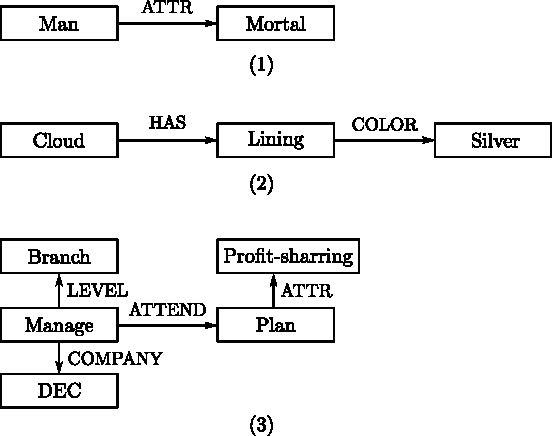
\includegraphics[scale=.9]{figures/ans-2.8.pdf}
		\caption{ 所求语义网络 } \label{Fig:semantic-net}
	\end{figure}
\end{solution}

\begin{question}
试构造一个描述你的寝室或办公室的框架系统。
\end{question}
\begin{solution}
以房间为例,如图\ref{Fig:semantic-my-room}。
	\begin{figure}[h]
		\centering
		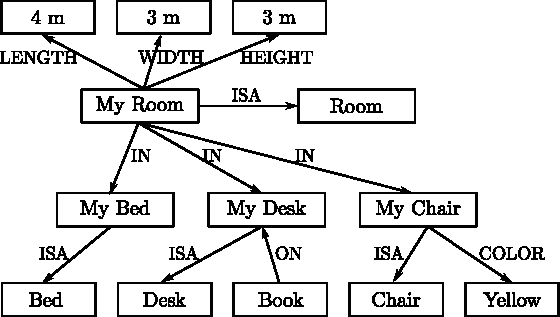
\includegraphics[scale=.9]{figures/ans-2.9.pdf}
		\caption{ 我的房间语义网络 } \label{Fig:semantic-my-room}
	\end{figure}
\end{solution}

\begin{question}
框架和本体有何关系与区别?
\end{question}
\begin{solution}
\end{solution}
\chapter{确定性推理}

\begin{question}
什么是图搜索过程?其中,重排OPEN表意味着什么?重排的原则是什么?
\end{question}	
\begin{solution}
图搜索的一般过程如下:
	\begin{enumerate}
		\item 建立一个只含有起始节点$S$的搜索图$G$,把$S$放到一个叫做OPEN的未扩展节点表中;
		\item 建立一个叫CLOSED的已扩展节点表,其初始为空表;
		\item LOOP:检查OPEN表是否为空,若为空,则失败退出;
		\item 选择OPEN表上的第一个节点,把它从OPEN表移出放进CLOSED表。并记该节点为节点$n$;
		\item 考察节点$n$是否为目标节点。若$n$为一目标节点,则有解并成功退出。此解是追踪图$G$中沿着指针从$n$到$S$这条路径而得到的(指针将在第7步中设置);
		\item 扩展节点$n$,生成一组子节点。把这些子节点中不是$n$的祖先的那些后继节点记入集合$M$。把$M$的这些成员作为$n$的后继节点添入图$G$中;
		\item 针对$M$中子节点的不同情况,分别作如下处理:
			\begin{itemize}
				\item 未曾在$G$中出现过的$M$成员设置一个通向其父节点(即节点$n$)的指针,并把$M$的这些成员加进OPEN表;(新生成的)
				\item 对已经在OPEN或CLOSED表上的每一个$M$成员,确定是否需要更改通到其父节点$n$的指针方向;(原生成但未扩展的)
				\item 对已在CLOSED表上的每个$M$成员,确定是否需要更改图$G$中通向它的每个后裔节点的指针方向;(原生成也扩展过的)
			\end{itemize}
		\item 按某一任意方式或按某个探试值,重排OPEN表;
		\item GO LOOP。
	\end{enumerate} \par
重排OPEN表意味着什么:在第(6)步中,将优先扩展哪个节点,不同的排序标准对应着不同的搜索策略。是否重新安排OPEN表,即是否按照某个试探值(或准则、启发信息等)重新对未扩展节点进行排序,将决定该图搜索过程是无信息搜索或启发式搜索。各种搜索策略的主要区别在于对OPEN表中节点的排列顺序不同。例如,广度优先搜索把先生成的子节点排在前面,而深度优先搜索则把后生成的子节点排在前面。\par
重排的原则当视具体需求而定,不同的原则对应着不同的搜索策略,如果想尽快地找到一个解,则应当将最有可能达到目标节点的那些节点排在OPEN表的前面部分,如果想找到代价最小的解,则应当按代价从小到大的顺序重排OPEN表。
\end{solution}

\begin{question}
试举例比较各种搜索方法的效率。
\end{question}	
\begin{solution}
几种搜索算法的效率:
	\begin{description}
		\item[宽度优先搜索] 只要问题有解,用宽度优先搜索总可以得到解,而且得到的是路径最短的解。宽度优先搜索盲目性较大,当目标节点距初始节点较远时将会产生许多无用节点,搜索效率低。
		\item[深度优先搜索] 搜索一旦进入某个分支,就将沿着该分支一直向下搜索。如果目标节点恰好在此分支上,则可较快地得到解。但是,如果目标节点不在此分支上,而该分支又是一个无穷分支,则就不可能得到解。所以深度优先搜索是不完备的,即使问题有解,它也不一定能求得解。所求得的解答路径不一定是最短路径。
		\item[有界深度优先搜索] 如果问题有解,且其路径长度$\leq dm$,则搜索过程一定能求得解。但是,若解的路径长度$> dm$,则搜索过程就得不到解。这说明在有界深度优先搜索中,深度界限的选择是很重要的。要恰当地给出$dm$的值是比较困难的。即使能求出解,它也不一定是最优解。
		\item[等代价搜索] 是宽度优先搜索的一种推广,不是沿着等长度路径断层进行扩展,而是沿着等代价路径断层进行扩展。搜索树中每条连接弧线上的有关代价,表示时间、距离等花费。若所有连接弧线具有相等代价,则简化为宽度优先搜索算法。
		\item[盲目搜索] 具有较大的盲目性,产生的无用节点较多,效率不高,耗费过多的计算空间与时间。
		\item[有序搜索] 利用启发信息,决定哪个是下一步要扩展的节点。选``最有希望''的节点作为下一个被扩展的节点。选择OPEN表上具有最小$f$值的节点作为下一个要扩展的节点, 又称为最佳优先搜索。正确选择估价函数对搜索结果具有决定性的作用。使用不能识别某些节点真实希望的估价函数会形成非最小代价路径;使用一个过多地估计了全部节点希望的估价函数又会扩展过多的节点。 
		\item[A算法] 虽提高了算法效率,但不能保证找到最优解。
		\item[A*算法] 搜索效率很大程度上取决于估价函数$h(n)$。一般来说,在满足$h(n)\leq h^*(n)$的前提下,$h(n)$的值越大越好。$h(n)$的值越大,说明它携带的启发性信息越多,A*算法搜索时扩展的节点就越少,搜索效率就越高。
	\end{description}

\end{solution}

\begin{question}
化为子句型有哪些步骤?请结合例子说明。
\end{question}	
\begin{solution}
任一谓词演算公式可以化成一个子句集。其变换过程由下列九个步骤组成:
	\begin{enumerate}
		\item 消去蕴涵符号,将蕴涵符号化为析取和否定符号;
		\item 减少否定符号的辖域,每个否定符号最多只用到一个谓词符号上,并反复应用狄·摩根定律;
		\item 对变量标准化,对哑元改名,以保证每个量词有其自己唯一的哑元;
		\item 消去存在量词,引入Skolem函数,消去存在量词。如果要消去的存在量词不在任何一个全称量词的辖域内,那么我们就用不含变量的Skolem函数即常量;
		\item 化为前束形,把所有全称量词移到公式的左边,并使每个量词的辖域包括这个量词后面公式的整个部分;
		\item 把母式化为合取范式, 反复应用分配律,将母式写成许多合取项的合取的形式,而每一个合取项是一些谓词公式和(或)谓词公式的否定的析取;
		\item 消去全称量词,消去前缀,即消去明显出现的全称量词;
		\item 消去连词符号(合取),用{合取项1, 合取项2}替换明显出现的合取符号;
		\item 更换变量名称,更换变量符号的名称,使一个变量符号不出现在一个以上的子句中。
	\end{enumerate}
\end{solution}

\begin{question}
如何通过消解反演求取问题的答案。
\end{question}	
\begin{solution}
给出一个公式集$S$和目标公式$L$,通过反证或反演来求证目标公式$L$,其证明步骤如下: 
	\begin{enumerate}
		\item 否定$L$,得$\sim L$; 
		\item 把$\sim L$添加到$S$中去; 
		\item 把新产生的集合$\left\{\sim L, S\right\}$化成子句集; 
		\item 应用消解原理,力图推导出一个表示矛盾的空子句。
	\end{enumerate}
\end{solution}

\begin{question}
什么叫合式公式?合式公式有哪些等价关系?
\end{question}	
\begin{solution}
合式公式的递归定义如下:
	\begin{enumerate}
		\item 原子谓词公式是合式公式。
		\item 若$A$为合式公式,则$\sim A$也是一个合式公式。
		\item 若$A$、$B$是合式公式,则$A \vee B$,$A \wedge B$、$A \to B$、$A \leftrightarrow B$也都是合式公式。
		\item 若$A$是合式公式,$x$为$A$中的自由变量,则$\left(\forall x\right) A$和$\left(\exists x\right) A$都是合式公式。
		\item 运用有限步上述规则(1)至(4)求得的那些公式是是合式公式。
	\end{enumerate}
等价关系有:
	\begin{enumerate}
		\item 否定之否定:$\sim(\sim P)=P$
		\item 蕴含与与或形式的等价:$\begin{cases}
		P\to Q = \sim P \vee Q\\
		\sim P\to Q = P \vee Q
		\end{cases}$ 
		\item 狄•摩根定律:$\begin{cases}
		\sim (P \vee Q) = \sim P \wedge \sim Q \\
		\sim (P \wedge Q) = \sim P \vee \sim Q 
		\end{cases}$
		\item 分配律:$\begin{cases}
		P \vee (Q \wedge R) = (P \vee Q) \wedge (P \vee R) \\
		P \wedge (Q \vee R) = (P \wedge Q) \vee (P \wedge R)
		\end{cases}$
		\item 交换律:$\begin{cases}
		P \vee Q = Q \vee P \\
		P \wedge Q = Q \wedge P
		\end{cases}$
		\item 结合律:$\begin{cases}
		P \vee (Q \vee R) = (P \vee Q) \vee R \\
		P \wedge (Q \wedge R) = (P \wedge Q) \wedge R
		\end{cases}$
		\item 逆否率:$(P \to Q) = (\sim Q \to \sim P)$
		\item 否定跨越量词:$\sim (\exists x) P(x) = (\forall x)[\sim P(x)]$
		\item 全称量词同与或连词:$\begin{cases}
		(\forall x)[P(x) \wedge Q(x)] = (\forall x) P(x) \wedge (\forall x) Q(x) \\
		(\forall x)[P(x) \vee Q(x)] = (\forall x) P(x) \vee (\forall x) Q(x)
		\end{cases}$
		\item 量词中的哑元:$\begin{cases}
		(\forall x) P(x) = (\forall y) P(y) \\
		(\exists x) P(x) = (\exists y) P(y)
		\end{cases}$
	\end{enumerate}
\end{solution}

\begin{question}
用宽度优先搜索求图\ref{Fig:maze}所示迷宫的出路。
	\begin{figure}[h]
		\centering
		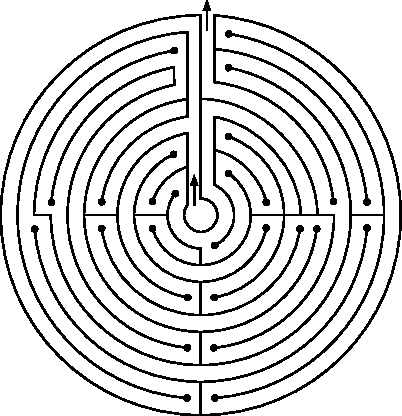
\includegraphics{figures/ques-3.6.pdf}
		\caption{迷宫一例} \label{Fig:maze}
	\end{figure}
\end{question}
\begin{solution}
在这个迷宫中,$S$是源节点,$F$是目标节点,$A$、$B$、$C$、$D$、$E$是$5$个具有二叉分支的节点,在每个节点处,都可能会出现两种路线,要么向左拐要么向右拐,我们在每个二叉节点处设立两个虚节点,以表示到该节点后的走向,向右拐为第一个虚节点,用下标$1$表示,向左拐为第二个虚节点,用下标$2$表示。例如,$A$节点处向右拐的虚节点用$A_1$表示,向左拐的虚节点用$A_2$表示。可以将该迷宫转换成一个有向图,如图\ref{Fig:maze-states-graph}。\par
	\begin{figure} [h]
		\centering
		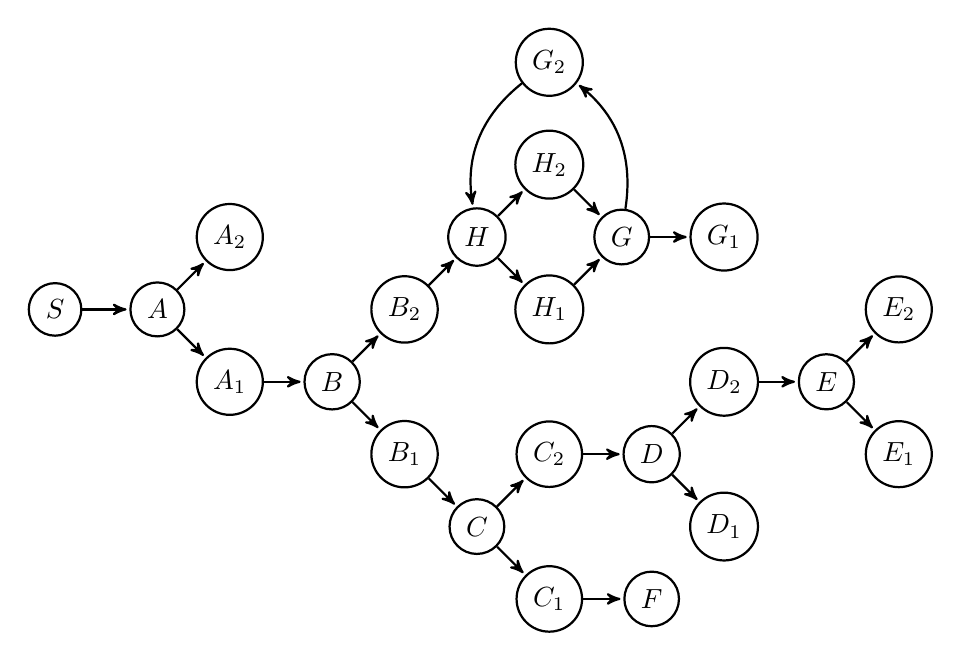
\begin{tikzpicture}[->,>=stealth',shorten >=1pt,auto,node distance=1.3cm,
                    thick,main node/.style={circle,draw}]

  \node[main node] (S) {$S$};
  \node[main node] (A) [right of=S] {$A$};
  \node[main node] (A2) [above right of=A] {$A_2$};
  \node[main node] (A1) [below right of=A] {$A_1$};
  \node[main node] (B) [right of=A1] {$B$};
  \node[main node] (B2) [above right of=B] {$B_2$};
  \node[main node] (H) [above right of=B2] {$H$};
  \node[main node] (H2) [above right of=H] {$H_2$};
  \node[main node] (H1) [below right of=H] {$H_1$};
  \node[main node] (G) [above right of=H1] {$G$};
  \node[main node] (G1) [right of=G] {$G_1$};
  \node[main node] (G2) [above of=H2] {$G_2$};
  \node[main node] (B1) [below right of=B] {$B_1$};
  \node[main node] (C) [below right of=B1] {$C$};
  \node[main node] (C2) [above right of=C] {$C_2$};
  \node[main node] (C1) [below right of=C] {$C_1$};
  \node[main node] (D) [right of=C2] {$D$};
  \node[main node] (D2) [above right of=D] {$D_2$};
  \node[main node] (D1) [below right of=D] {$D_1$};
  \node[main node] (E) [right of=D2] {$E$};
  \node[main node] (E2) [above right of=E] {$E_2$};
  \node[main node] (E1) [below right of=E] {$E_1$};
  \node[main node] (F) [right of=C1] {$F$};
  

  \path[every node/.style={}]
  	(S) edge (A)
  	(A) edge (A1)
  		edge (A2)
  	(A1) edge (B)
  	(B) edge (B1)
  		edge (B2)
  	(B2) edge (H)
  	(H) edge (H1)
  		edge (H2)
  	(H2) edge (G)
  	(H1) edge (G)
  	(G) edge (G1)
  		edge [bend right] (G2)
  	(G2) edge [bend right] (H)
  	(B1) edge (C)
  	(C) edge (C1)
  		edge (C2)
  	(C2) edge (D)
  	(D) edge (D1)
  		edge (D2)
  	(D2) edge (E)
  	(E) edge (E1)
  		edge (E2)
  	(C1) edge (F);
\end{tikzpicture}
		\caption{迷宫状态空间图} \label{Fig:maze-states-graph}
	\end{figure}
除F节点是目标节点外,其余没有后继节点的虚节点都说明走入了死胡同。\par
利用深度优先搜索,其搜索树如图\subref*{Fig:maze-search-graph-dfs}所示,图中节点旁所标数字为节点扩展次序。所得到的解路径为:
\[ S \to A \to A_1 \to B \to B_1 \to C \to C_1 \to F \]
也就是说,从S出发,在A节点处不能左拐,而是直行,到B节点处右拐,到C节点也右拐,即可到达出口F。\par
利用宽度优先搜索,其搜索树如图\subref*{Fig:maze-search-graph-bfs}所示,图中节点旁所标数字为节点扩展次序。所得到的解路径为:
\[ S \to A \to A_1 \to B \to B_1 \to C \to C_1 \to F \]
由搜索过程可以看出,宽度优先搜索的效率低于深度优先搜索。
	\begin{figure} [h]
		\centering
		\captionsetup{justification=raggedright}
		\subfloat[深度优先搜索]{\label{Fig:maze-search-graph-dfs}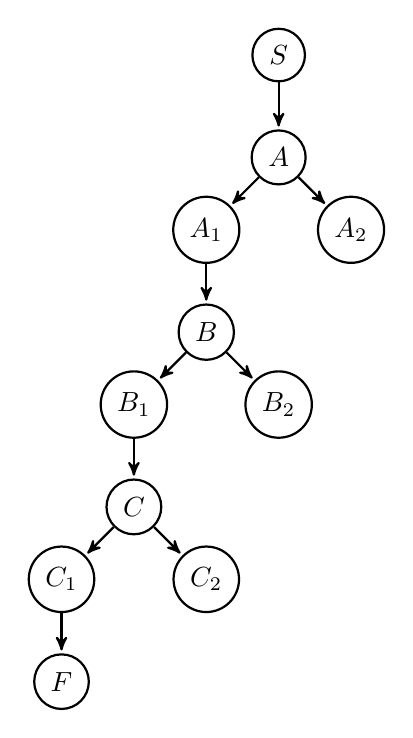
\begin{tikzpicture}[->,>=stealth',shorten >=1pt,auto,node distance=1.3cm,
                    thick,main node/.style={circle,draw}]

  \node[main node] (S) {$S$};
  \node[main node] (A) [below of=S] {$A$};
  \node[main node] (A1) [below left of=A] {$A_1$};
  \node[main node] (A2) [below right of=A] {$A_2$};
  \node[main node] (B) [below of=A1] {$B$};
  \node[main node] (B1) [below left of=B] {$B_1$};
  \node[main node] (B2) [below right of=B] {$B_2$};
  \node[main node] (C) [below of=B1] {$C$};
  \node[main node] (C1) [below left of=C] {$C_1$};
  \node[main node] (C2) [below right of=C] {$C_2$};
  \node[main node] (F) [below of=C1] {$F$};
  

  \path[every node/.style={}]
  	(S) edge (A)
  	(A) edge (A1)
  		edge (A2)
  	(A1) edge (B)
  	(B) edge (B1)
  		edge (B2)
  	(B1) edge (C)
  	(C) edge (C1)
  		edge (C2)
  	(C1) edge (F);
\end{tikzpicture}}\qquad
		\subfloat[宽度优先搜索]{\label{Fig:maze-search-graph-bfs}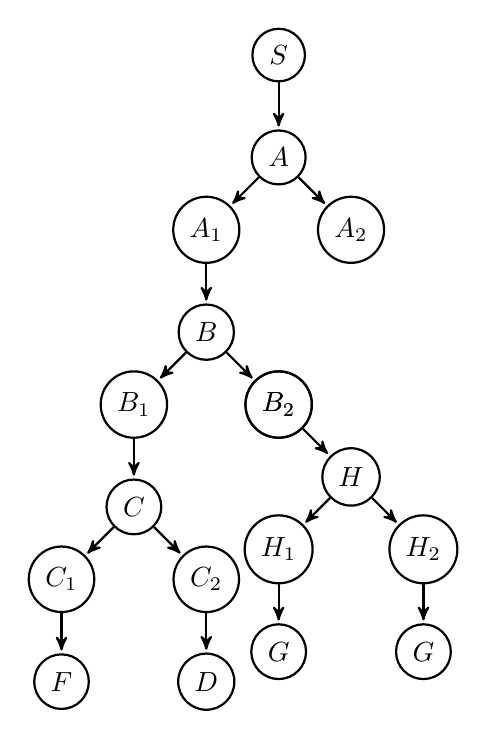
\begin{tikzpicture}[->,>=stealth',shorten >=1pt,auto,node distance=1.3cm,
                    thick,main node/.style={circle,draw}]

  \node[main node] (S) {$S$};
  \node[main node] (A) [below of=S] {$A$};
  \node[main node] (A1) [below left of=A] {$A_1$};
  \node[main node] (A2) [below right of=A] {$A_2$};
  \node[main node] (B) [below of=A1] {$B$};
  \node[main node] (B1) [below left of=B] {$B_1$};
  \node[main node] (B2) [below right of=B] {$B_2$};
  \node[main node] (C) [below of=B1] {$C$};
  \node[main node] (C1) [below left of=C] {$C_1$};
  \node[main node] (C2) [below right of=C] {$C_2$};
  \node[main node] (F) [below of=C1] {$F$};
  \node[main node] (D) [below of=C2] {$D$};
  \node[main node] (B2) [below right of=B] {$B_2$};
  \node[main node] (H) [below right of=B2] {$H$};
  \node[main node] (H1) [below left of=H] {$H_1$};
  \node[main node] (H2) [below right of=H] {$H_2$};
  \node[main node] (G) [below of=H1] {$G$};
  \node[main node] (G') [below of=H2] {$G$};
  

  \path[every node/.style={}]
  	(S) edge (A)
  	(A) edge (A1)
  		edge (A2)
  	(A1) edge (B)
  	(B) edge (B1)
  		edge (B2)
  	(B2) edge (H)
  	(H) edge (H1)
  		edge (H2)
  	(H1) edge (G)
  	(H2) edge (G')
  	(B1) edge (C)
  	(C) edge (C1)
  		edge (C2)
  	(C1) edge (F)
  	(C2) edge (D);
\end{tikzpicture}}
	    \caption{迷宫搜索图}
	\end{figure}
\end{solution}

\begin{question}
用有界深度优先搜索方法求解图\ref{Fig:8-code}所示八数码难题。
	\begin{figure}[H]
		\centering
		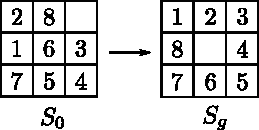
\includegraphics{figures/ques-3.7.pdf}
		\caption{八数码难题} \label{Fig:8-code}
	\end{figure}
\end{question}
\begin{solution}
定义操作符集:$F=\{f1,f2,f3,f4\}$,其中:$f1$表示空格右移;$f2$表示空格上移;$f3$表示空格左移;$f4$表示空格下移。\par
搜索时,节点的扩展顺序规定为按右、左、上、下方向移动空格。并设置深度界限为$8$。\par
	\begin{figure}[H]
		\centering
		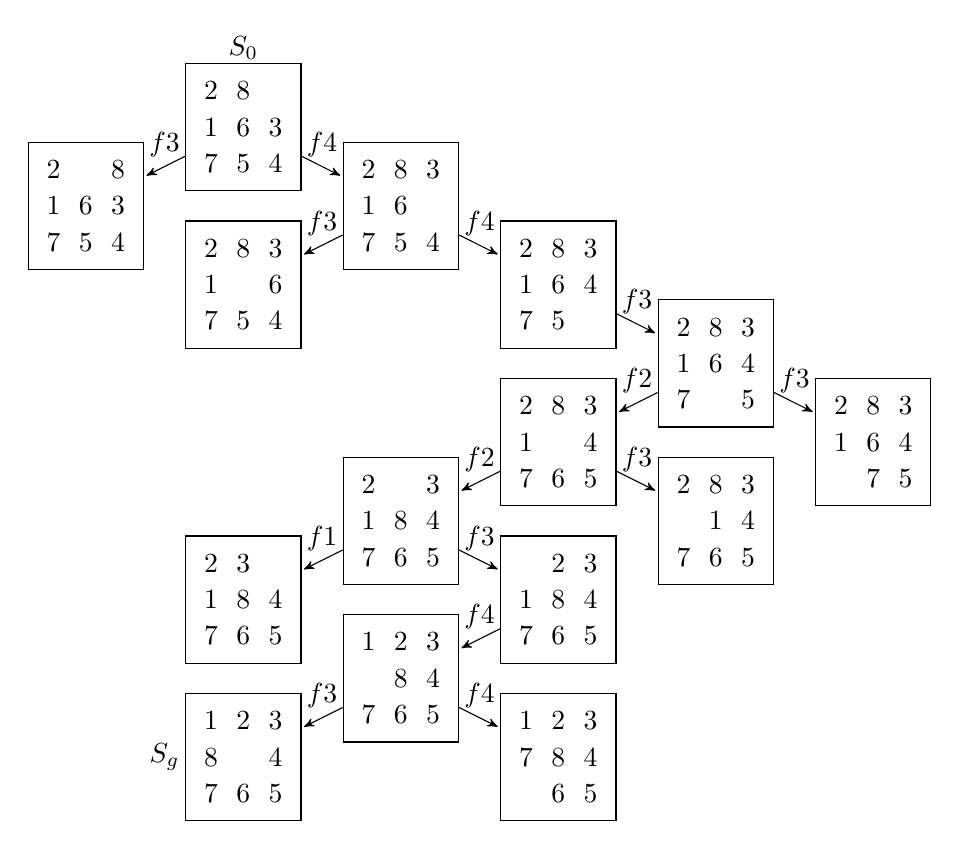
\begin{tikzpicture}[->,>=stealth',shorten >=1pt, every node/.append style={on grid,node distance=1cm and 2cm},
                    every matrix/.append style={matrix of nodes,draw}]

\matrix (0) at(0,0) {2&8&\,\\ 1&6&3\\ 7&5&4\\};
\matrix [below left=of 0] (1) {2&\,&8\\ 1&6&3\\ 7&5&4\\};
\matrix [below right=of 0] (2) {2&8&3\\ 1&6&\,\\ 7&5&4\\};
\matrix [below left=of 2] (3) {2&8&3\\ 1&\,&6\\ 7&5&4\\};
\matrix [below right=of 2] (4) {2&8&3\\ 1&6&4\\ 7&5&\,\\};
\matrix [below right=of 4] (5) {2&8&3\\ 1&6&4\\ 7&\,&5\\};
\matrix [below left=of 5] (6) {2&8&3\\ 1&\,&4\\ 7&6&5\\};
\matrix [below right=of 5] (7) {2&8&3\\ 1&6&4\\ \,&7&5\\};
\matrix [below left=of 6] (8) {2&\,&3\\ 1&8&4\\ 7&6&5\\};
\matrix [below right=of 6] (9) {2&8&3\\ \,&1&4\\ 7&6&5\\};
\matrix [below left=of 8] (10) {2&3&\,\\ 1&8&4\\ 7&6&5\\};
\matrix [below right=of 8] (11) {\,&2&3\\ 1&8&4\\ 7&6&5\\};
\matrix [below left=of 11] (12) {1&2&3\\ \,&8&4\\ 7&6&5\\};
\matrix [below left=of 12] (13) {1&2&3\\ 8&\,&4\\ 7&6&5\\};
\matrix [below right=of 12] (14) {1&2&3\\ 7&8&4\\ \,&6&5\\};
\node [above=of 0] {$S_0$};
\node [left= 1cm of 13]{$S_g$};

\draw (0) edge node[above]{$f3$} (1) 
          edge node[above]{$f4$} (2);
\draw (2) edge node[above]{$f3$} (3)
          edge node[above]{$f4$} (4);
\draw (4) edge node[above]{$f3$} (5);
\draw (5) edge node[above]{$f2$} (6)
          edge node[above]{$f3$} (7);
\draw (6) edge node[above]{$f2$} (8)
          edge node[above]{$f3$} (9);
\draw (8) edge node[above]{$f1$} (10)
          edge node[above]{$f3$} (11);
\draw (11) edge node[above]{$f4$} (12);
\draw (12) edge node[above]{$f3$} (13)
           edge node[above]{$f4$} (14);

\end{tikzpicture}
		\caption{八数码难题} \label{Fig:8-digits-search-dfs}
	\end{figure}
由图\ref{Fig:8-digits-search-dfs}有界深度优先搜索树中可见,当$d=8$时,八数码难题的一个解为:
\[f4, f4, f3, f2, f2, f3, f4, f3 \, .\]
\end{solution}

\begin{question}
应用最新的方法表达传教士和野人问题,编写一个计算机程序,以求得安全渡过全部$6$个人的解答。(提示:在应用状态空间表示和搜索方法时,可用$(N_m,N_c)$来表示状态描述,其中$N_m$和$N_c$分别为传教士和野人的人数。初始状态为$(3,3)$,而可能的中间状态为$(0,1)$,$(0,2)$,$(0,3)$,$(1,1)$,$(2,1)$,$(2,2)$,$(3,0)$,$(3,1)$和$(3,2)$等。
\end{question}
\begin{solution}
略。
\end{solution}

\begin{question}
试比较宽度优先搜索、有界深度优先搜索及有序搜索的搜索效率,并以实例数据加以说明。
\end{question}
\begin{solution}
以八数码难题为例,下面比较宽度优先搜索、有界深度优先搜索及有序搜索的搜索效率。\par
	\begin{table}[htbp]
	\centering
	\begin{tabular}{p{50pt}p{40pt}p{40pt}p{140pt}}
		\toprule
		搜索方法 & CLOSE表长度 & OPEN表长度 & 搜索效率 \\
		\midrule
		宽度优先搜索 & 27 & 11 &
		优点:只要问题有解,总可以得到解,而且得到的是路径最短的解。\newline 缺点:盲目性较大,当目标节点距初始节点较远时将会产生许多无用节点,搜索效率低。 \\
		\midrule
		有界深度优先搜索 & 16 & 13 &
		如果问题有解,且其路径长度$\leq d_m$,则上述搜索过程一定能求得解。但是,若解的路径长度$>d_m$,则上述搜索过程就得不到解。这说明在有界深度优先搜索中,深度界限的选择是很重要的。要恰当地给出$d_m$的值是比较困难的。即使能求出解,它也不一定是最优解。\newline 搜索效率低。 \\
		\midrule
		有序搜索 & 5 & 7 &
		宽度优先搜索、深度优先搜索、等代价搜索均是有序搜索技术的特例。正确选择估价函数对搜索结果具有决定性的作用。\newline 搜索效率高。\\
		\bottomrule
	\end{tabular}
	\caption{搜索效率比较}\label{tab:comparison-of-searching}
	\end{table} 
\end{solution}

\begin{question}
一个机器人驾驶卡车,携带包裹(编号分别为\#1、\#2和\#3)分别投递到林(LIN)、吴(WU)和胡(HU) 3家住宅处。规定了某些简单的操作符,如表示驾驶方位的$\mathrm{drive}(x,y)$和表示卸下包裹的$\mathrm{unload}(z)$;对于每个操作符,都有一定的先决条件和结果。试说明状态空间问题求解系统如何能够应用谓词演算求得一个操作符序列,该序列能够生成一个满足$\mathrm{AT(\# 1,LIN) \wedge AT(\# 2,WU) \wedge AT(\# 3,HU)}$的目标状态。
\end{question}
\begin{solution}
初始状态可描述为:
	\begin{multline*}
	\mathrm{AT}(\#1, \sim \mathrm{LIN}) \wedge \mathrm{AT}(\#2, \sim \mathrm{WU}) \wedge \mathrm{AT}(\#3, \sim \mathrm{HU}) \wedge {} \\
	\mathrm{AT}(\#1, \mathrm{CAR}) \wedge \mathrm{AT}(\#2, \mathrm{CAR}) \wedge \mathrm{AT}(\#3, \mathrm{CAR})
	\end{multline*} 
目标状态可描述为:
	\begin{multline*}
	\mathrm{AT}(\#1, \mathrm{LIN}) \wedge \mathrm{AT}(\#2, \mathrm{WU}) \wedge \mathrm{AT}(\#3, \mathrm{HU}) \wedge {} \\
	\mathrm{AT}(\#1, \sim \mathrm{CAR}) \wedge \mathrm{AT}(\#2, \sim \mathrm{CAR}) \wedge \mathrm{AT}(\#3, \sim \mathrm{CAR})
	\end{multline*}
对每个操作符都有一定的先决条件和结果,如表\ref{tab:operators}:
	\begin{table}[htbp]
	\centering
	\begin{tabular}{p{50pt}p{130pt}p{130pt}}
		\toprule
		~ & 先决条件 & 结果 \\
		\midrule
		$\mathrm{drive}(x,y)$ & $\mathrm{AT}(\mathrm{CAR}, x)$ & $\mathrm{AT}(\mathrm{CAR}, y)$ \\
		\midrule
		$\mathrm{unload}(z)$ & $\mathrm{AT}(z, \mathrm{CAR}) \wedge \mathrm{AT}(\mathrm{CAR}, x)$ 
			& $\mathrm{AT}(z, \sim\mathrm{CAR}) \wedge \mathrm{AT}(x, x)$ \\
		\bottomrule
	\end{tabular}
	\caption{每个操作符的先决条件和结果}\label{tab:operators}
	\end{table} \par
至此,原问题就转换为:寻找一个可将初始状态转换到目标状态的操作序列,如何求得该操作序列。
\end{solution}

\begin{question}
规则演绎系统和产生式系统有哪几种推理方式?各自的特点为是什么?
\end{question}
\begin{solution}
规则演绎系统的推理方式有正向推理、逆向推理和双向推理。正向推理、逆向推理的特点见表\ref{tab:reasoning-of-rule-based-system};双向推理组合了正向推理和逆向推理的优点,克服了各自的缺点,具有更高的搜索求解效率。
	\begin{table}[htbp]
	\centering
	\begin{tabular}{p{80pt}p{110pt}p{110pt}}
		\toprule
		~ & 正向推理 & 逆向推理 \\
		\midrule
		推理方向 & 从if部分向then部分推理的过程,它是从事实或状况向目标或动作进行操作的 & 从then部分向if部分推理的过程,它是从目标或动作向事实或状况进行操作的 \\
		\midrule
		目标表达式 & 文字的析取 & 任意形式 \\
		\midrule
		事实表达式 & 任意形式 & 文字的合取 \\
		\bottomrule
	\end{tabular}
	\caption{规则演绎系统系统的推理方式}\label{tab:reasoning-of-rule-based-system}
	\end{table} 
	\par
产生式系统的推理方式有正向推理、逆向推理和双向推理。正向推理、逆向推理的特点见表\ref{tab:reasoning-of-production-system};双向推理结合了正向推理和逆向推理的长处,克服了两者的短处,其控制策略比两者都要复杂。
	\begin{table}[htbp]
	\centering
	\begin{tabular}{p{80pt}p{110pt}p{110pt}}
		\toprule
		~ & 正向推理 & 逆向推理 \\
		\midrule
		驱动方式 & 数据驱动 & 目标驱动 \\ 
		\midrule
		推理方法 & 从一组数据出发向前推到结论 & 从可能的解答出发,向后推理验证解答 \\ 
		\midrule
		启动方法 & 从一个事件启动 & 由询问关于目标状态的一个问题而启动 \\ 
		\midrule
		透明程度 & 不能解释其推理过程 & 可解释其推理过程 \\ 
		\midrule
		推理方向 & 由底向上推理 & 由顶向下推理 \\ 
		\midrule
		优点 & 算法简单、容易实现,允许用户一开始就把有关的事实数据存入数据库,在执行过程中系统能很快获得这些数据,而不必等到系统需要数据时才向用户询问 & 搜索目的性强,推理效率高 \\ 
		\midrule
		缺点 & 盲目搜索,可能会求解许多与总目标无关的子目标,每当总数据库内容更新后都要遍历整个规则库,推理效率较低 & 目标的选择具有盲目性,可能会求解许多假的目标;当可能的结论数目很多,即目标空间很大时,推理效率不高;当规则的右部是执行某种动作不是结论时,逆向推理不便使用 \\ 
		\midrule
		适用场合 & 主要用于已知初始数据,而无法提供推理目标,或解空间很大的一类问题,如监控、预测、规划、设计等问题的求解 & 主要用于结论单一或者已知目标结论,而要求验证的系统,如选择、分类、故障诊断等问题的求解 \\ 
		\midrule
		典型系统 & CLIPS,OPS & PROLOG \\
		\bottomrule
	\end{tabular}
	\caption{产生式系统的推理方式}\label{tab:reasoning-of-production-system}
	\end{table}
\end{solution}

\begin{question}
单调推理有何局限性?什么叫缺省推理?非单调推理系统如何证实一个节点的有效性?
\end{question}
\begin{solution}
单调系统不能很好地处理常常出现在现实问题领域中的3类情况,即不完全的信息、不断变化的情况、以及求解复杂问题过程中生成的假设。有两种方法可以证实节点的有效性:
	\begin{enumerate}
		\item 支持表。(SL (IN-节点表) (OUT-节点表)) \\
			如果某节点的IN节点表中提到的节点当前都是IN, 且OUT节点表中提到的节点当前都是OUT,则它是有效的。
		\item 条件证明。(CP(结论) (IN-假设) (OUT-假设)) \\
			条件证明(CP)的证实表示有前提的论点,无论何时,只要在IN假设中的节点为IN,OUT假设中的节点为OUT,则结论节点往往为IN,于是条件证明的证实有效。 
	\end{enumerate}
\end{solution}

\begin{question}
在什么情况下需要采用不确定推理或非单调推理?
\end{question}
\begin{solution}
不完全的信息、不断变化的情况、以及求解复杂问题过程中生成的假设。
\end{solution}

\begin{question}
下列语句是一些几何定理,把这些语句表示为基于规则的几何证明系统的产生式规则:
	\begin{enumerate}
		\item 两个全等三角形的各对应角相等。
		\item 两个全等三角形的各对应边相等。 
		\item 各对应边相等的三角形是全等三角形。
		\item 等腰三角形的两底角相等。 
	\end{enumerate}
\end{question}
\begin{solution}
产生式规则如下:
	\begin{enumerate}
		\item IF 两个三角形全等 THEN 各对应角相等;
		\item IF 两个三角形全等 THEN 各对应边相等;
		\item IF 两个三角形各对应边相等 THEN 两三角形全等;
		\item IF 它是等腰三角形 THEN 它的两底角相等。
	\end{enumerate}
\end{solution}
\chapter{非经典推理}


\chapter{计算智能}

\begin{question}
计算智能的含义是什么?它涉及哪些研究分支?
\end{question}
\begin{solution}
贝兹德克认为计算智能取决于制造者提供的数值数据,而不依赖于知识;另一个方面,人工智能则应用知识精品。计算智能是一种智力方式的低层认知,它与人工智能的区别只是认知层次从中层下降至底层而已。中层系统含有知识(精品),底层系统则没有。它与人工智能的主要区别在于它不含知识精品。\par
计算智能主要的研究领域为神经计算,模糊计算,进化计算,人工生命。 
\end{solution}

\begin{question}
试述计算智能(CI)、人工智能(AI)和生物智能(BI)的关系。
\end{question}
\begin{solution}
计算智能是智力的低层认知,主要取决于数值数据而不依赖于知识。人工智能是在计算智能的基础上引入知识而产生的智力中层认知。生物智能,尤其是人类智能,则是最高层的智能。\par
A- Artificial,表示人工的(非生物的);\par
B- Biological,表示物理的+化学的+(?)=生物的;\par
C- Computational,表示数学+计算机。\par
CI智能是最低的,它没有知识,就是数据计算。从复杂性来看,BI$>$AI$>$CI;从所属关系来看,CI$\subset$AI$\subset$BI;AI是CI到BI的过渡,因为AI中除计算算法之外,还包括符号表示及数值信息处理。\par
计算智能是一种智力方式的低层认知,它与人工智能的区别只是认知层次从中层下降至低层而已。中层系统含有知识,低层系统则没有。
\end{solution}

\begin{question}
人工神经网络为什么具有诱人的发展前景和潜在的广泛应用领域?
\end{question}
\begin{solution}
人工神经网络具有如下至关重要的特性:
	\begin{enumerate}
		\item 并行分布处理 \\
神经网络具有高度的并行结构和并行实现能力,因为具有较好的耐故障能力和较快的总体处理能力。这一特性特别适于实时和动态处理。
		\item 非线性映射 \\
神经网络具有固有的非线性特性,这源于其近似任意非线性映射(变换)能力。这一特性给处理非线性问题带来新的希望。
		\item 通过训练进行学习 \\
神经网络是通过所研究系统过去的数据记录进行训练的。一个经过适当训练的神经网络具有归纳全部数据的能力。因此,神经系统能够解决那些由数学模型或描述规则难以处理的问题。
		\item 适应与集成 \\
神经网络能够适应在线运行,并能同时进行定量和定性操作。神经网络的强适应和信息融合能力使得它可以同时输入大量不同的控制信号,解决输入信息间的互补和冗余问题,实现信息集成和融合处理。这些特性特别适于复杂、大规模和多变量系统。
		\item 硬件实现 \\
神经网络不仅能够通过软件而且可以借助硬件实现并行处理。近年来,一些超大规模集成电路实现硬件已经问世,而且可以从市场上购买到。这使得神经网络成为具有快速和大规模处理能力的网络。
	\end{enumerate} \par
	显然,神经网络由于其学习和适应、自组织、函数逼近和大规模并行处理等能力,因而具有用于智能系统的潜力。\par
	神经网络在模式识别、信号处理、系统辨识和优化等方面的应用,已有广泛研究。在控制领域,已经做出许多努力,把神经网络用于控制系统,处理控制系统的非线性和不确定性以及逼近系统的辨识函数等。
\end{solution}

\begin{question}
简述生物神经元及人工神经网络的结构和主要学习算法。
\end{question}
\begin{solution}
生物神经元的结构:\par
大多数神经元由一个细胞体(cell body或soma)和突触(process)两部分组成。突触分两类, 即轴突(axon)和树突(dendrite),轴突是个突出部分,长度可达1m,把本神经元的输出发送至其它相连接的神经元。树突也是突出部分,但一般较短,且分枝很多,与其它神经元的轴突相连,以接收来自其它神经元的生物信号。\par
轴突的末端与树突进行信号传递的界面称为突触(synapse),通过突触向其它神经元发送信息。对某些突触的刺激促使神经元触发(fire)。只有神经元所有输入的总效应达到阈值电平,它才能开始工作。此时,神经元就产生一个全强度的输出窄脉冲,从细胞体经轴突进入轴突分枝。这时的神经元就称为被触发。突触把经过一个神经元轴突的脉冲转化为下一个神经元的兴奋或抑制。学习就发生在突触附近。\par
每个人脑大约含有1011-1012个神经元,每一神经元又约有103-104个突触。神经元通过突触形成的网络,传递神经元间的兴奋与抑制。大脑的全部神经元构成极其复杂的拓扑网络群体,用于实现记忆与思维。\par
人工神经网络的结构:\par
人工神经网络由神经元模型构成。每个神经元具有单一输出,并且能够与其它神经元连接,存在许多输出连接方法,每种连接方法对应于一个连接权系数。人工神经网络的结构分为2类:
	\begin{enumerate}
	\item 递归(反馈)网络 \\
有些神经元的输出被反馈至同层或前层神经元。信号能够从正向和反向流通。Hopfield网络,Elmman网络和Jordan网络是代表。 
	\item 前馈网络 \\
具有递阶分层结构,由一些同层神经元间不存在互连的层级组成。从输入层至输出层的信号通过单向连接流通,神经元从一层连接至下一层,不存在同层神经元之间的连接。多层感知器(MLP),学习矢量量化网络(LVQ),小脑模型连接控制网络(CMAC)和数据处理方法网络(GMDH)是代表。
	\end{enumerate} \par
人工神经网络的主要学习算法:
	\begin{enumerate}
	\item 指导式(有师)学习 \\
根据期望和实际的网络输出之间的差来调整神经元连接的强度或权。包括Delta规则,广义Delta规则,反向传播算法及LVQ算法。 
	\item 非指导(无导师)学习 \\
训练过程中,神经网络能自动地适应连接权,以便按相似特征把输入模式分组聚集。包括Kohonen算法,Carpenter-Grossberg自适应谐振理论(ART)。 
	\item 强化学习 \\
是有师学习的一种特例。它不需要老师给出目标输出,而是由一个“评论员”来评介与给定输入相对应的神经网络输出的优度。例如遗传算法(GA)。  
	\end{enumerate}	 
\end{solution}

\begin{question}
考虑一个具有阶梯形阈值函数的神经网络,假设
	\begin{enumerate}
		\item 用一常数乘所有的权值和阈值;
		\item 用一常数加所有的权值和阈值。
	\end{enumerate}
试说明网络性能是否会变化?
\end{question}
\begin{solution}
	\begin{enumerate}
		\item 不会。
		\item 会。
	\end{enumerate}
\end{solution}

\begin{question}
构作一个神经网络,用于计算含有两个输入的XOR函数。指定所用神经网络单元的种类。
\end{question}
\begin{solution}
已知用单层感知机是无法解决XOR问题的,需要增加隐单元。隐单元的数量可以有多种选择。这里给出含有两个隐单元(只有一层隐单元)的前馈神经网络。\par 
	\begin{figure}[h]
		\centering
		\def\layersep{2.5cm}

\begin{tikzpicture}[shorten >=1pt,->,draw=black, node distance=\layersep,
	every edge/.append style={nodes={font=\scriptsize}}]
    \tikzstyle{every pin edge}=[<-,shorten <=1pt]
    \tikzstyle{neuron}=[circle,draw=black,minimum size=17pt,inner sep=0pt]
    \tikzstyle{input neuron}=[neuron];
    \tikzstyle{output neuron}=[neuron];
    \tikzstyle{hidden neuron}=[neuron];
    \tikzstyle{annot} = [text width=4em, text centered]

    % Draw the input layer nodes
    %\foreach \name / \y in {1,...,2}
    % This is the same as writing \foreach \name / \y in {1/1,2/2,3/3,4/4}
        \node[input neuron, pin=left:] (I-1) at (0,-1) {$a$};
        \node[input neuron, pin=left:] (I-2) at (0,-2) {$b$};

    % Draw the hidden layer nodes
    %\foreach \name / \y in {1,...,2}
        \node[hidden neuron] (H-1) at (\layersep,-1 cm) {$c$};
        \node[hidden neuron] (H-2) at (\layersep,-2 cm) {$d$};

    % Draw the output layer node
    \path[yshift=0.5cm]
    		node[output neuron,pin={[pin edge={->}]right:}, right of=H-1, yshift=-0.5cm] (O) {$e$};

    % Connect every node in the input layer with every node in the
    % hidden layer.    
    \path (I-1) edge node[sloped, above]{$1$} (H-1);
    \path (I-1) edge node[sloped, below right= 0pt and 1pt]{$0.5$} (H-2);
    \path (I-2) edge node[sloped, above right= 0pt and 1pt]{$1$} (H-1);
    \path (I-2) edge node[sloped, below]{$0.5$} (H-2);

    % Connect every node in the hidden layer with the output layer
    \path (H-1) edge node[sloped, above]{$1$} (O);
    \path (H-2) edge node[sloped, below]{$-1$} (O);

    % Annotate the layers
    \node[annot,above of=H-1, node distance=1cm] (hl) {隐含层};
    \node[annot,left of=hl] {输入层};
    \node[annot,right of=hl] {输出层};

\end{tikzpicture}
		\caption{XOR问题的神经网络} \label{Fig:NN-XOR}
	\end{figure}
支持XOR问题的神经网络可以如图\ref{Fig:NN-XOR}所示。在这个神经网络中,共有5个处理单元,其中,$a$和$b$是输入单元,$c$和$d$是隐单元,它们位于网络的同一层上,$e$是输出单元。各单元的作用函数$O_i = f(a_i)$为阈值型。
\[O_i = \begin{cases}
	1, \quad a_i \geq 1 \\
	0, \quad a_i < 1
\end{cases} \]
\end{solution}

\begin{question}
假定有个具有线性激励函数的神经网络,即对于每个神经元,其输出等于常数$c$乘以各输入加权和。
	\begin{enumerate}
		\item 设该网络有个隐含层。对于给定的权$W$,写出输出层单元的输出值,此值以权$W$和输入层$I$为函数,而对隐含层的输出没有任何明显的叙述。试证明:存在一个不含隐含单位的网络能够计算上述同样的函数。
		\item 对于具有任何隐含层数的网络,重复进行上述计算。从中给出线性激励函数的结论。
	\end{enumerate}
\end{question}
\begin{solution}
为简单起见,这里假设在每个单元激励函数为相同的线性函数:$g(x)=cx+d$(如果对每个单元允许不同的$c_i$和$d_i$是一样的)。
	\begin{enumerate}
	\item 隐含层的输出为
	\[ H_j = g \left( \sum\limits_k W_{kj} I_k \right) = c \sum\limits_k W_{kj} I_k + d \, ,\]
	最终的输出为
	\[ O_i = g \left( \sum\limits_j W_{ji} H_j \right) = c \left( \sum\limits_j W_{ji} \left( c \sum\limits_k W{kj} I_k + d \right) \right) + d \, ,\]
	对于该输出,可以看出实际上可以化为输入的线性关系:
	\[ O_i = c^2 \sum\limits_k I_k \sum\limits_j W_{kj} W_{ji} + d \left( 1 + c \sum\limits_j W_{ji} \right) 、, . \]
	这样,就可以只使用一层感知机计算和两层网络相同的函数,其权重和激励函数分别为:
	\[ W_{ki} = \sum\limits_j W_{kj} W_{ji} \, ,\]
	\[ g(x) = c^2 + d \left( 1+c \sum\limits_j W_{ji} \right) \, .\]
	\item 上述归约可以将n层网络归约为$n-1$网络。归纳得出,n层网络可以归约为单层网络。这样,线性激励函数使得神经网络只能表示线性的函数。
	\end{enumerate}
\end{solution}

\begin{question}
什么是模糊性?它的对立含义是什么?试各举出两个例子加以说明。
\end{question}
\begin{solution}
模糊性指的是事物特性未被真实展现。它的对立含义是客观真实性。比如人到中年具有模糊性,人们对``中年''的理解并不是精确的一个岁数。58岁是一个精确的岁数。
\end{solution}

\begin{question}
什么是模糊集合和隶属函数或隶属度?
\end{question}
\begin{solution}
模糊集合是用来表达模糊性概念的集合,又称模糊集、模糊子集。设$U$为某些对象的集合,称为论域,可以是连续的或离散的;$u$表示$U$的元素,记作$U={u}$。论域$U$到$[0,1]$区间的任一映射$\mu_F$,即$\mu_F \colon U\to [0,1]$,都确定U的一个模糊子集$F$;$\mu_F$称为$F$的隶属函数或隶属度。
\end{solution}

\begin{question}
模糊集合有哪些运算?满足哪些规律?
\end{question}
\begin{solution}
模糊集合的交、并、补。设$A$、$B$是论域$U$上的两个模糊集,分别称$A \cup B$、$A \cap B$为$A$与$B$的并集、交集,称$\overline{A}$为$A$的补集,它们的隶属函数分别为:
	\begin{align*}
		\mu_{A \cup B}(u) &= \max \left\{ \mu_A(u), \mu_B(u) \right\} \\
		\mu_{A \cap B}(u) &= \min \left\{ \mu_A(u), \mu_B(u) \right\} \\
		\mu_{\overline{A}} &= 1 - \mu_A(u)
	\end{align*}
\end{solution}

\begin{question}
什么是模糊推理?
\end{question}
\begin{solution}
模糊推理是建立在模糊逻辑基础上的,一种不确定性推理方法,是在二值逻辑三段论基础上发展起来的。它以模糊判断为前提,动用模糊语言规则,推导出一个近似的模糊判断结论。\par
推理方法有Zadeh法、Baldwin法、Tsukamoto法和Mizumoto法等方法。在Zadeh法中,有2种重要的模糊推理规则:广义取式(肯定前提)假言推理法(GMP)和广义拒式(否定结论)假言推理法(GMT),分别简称为广义前向推理法和广义后向推理法。  
\end{solution}

\begin{question}
对某种产品的质量进行抽查评估。现随机选出5个产品$x_1$,$x_2$,$x_3$,$x_4$,$x_5$进行检验,它们质量情况分别为:
\[ x_1=80, x_2=72, x_3=65, x_4=98, x_5=53\]
这就确定了一个模糊集合$Q$,表示该组产品的``质量水平''这个模糊概念的隶属程度。
试写出该模糊集。
\end{question}
\begin{solution}
该模糊集为$Q={(x_1,0.8), (x_2, 0.72), (x_3,0.65), (x_4,0.98), (x_5,0.53)}$。
\end{solution}

\begin{question}
试述遗传算法的基本原理,并说明遗传算法的求解步骤。
\end{question}
\begin{solution}
遗传算法的基本原理是,通过随机方式产生若干个所求解问题的数字编码,即染色体,形成初始种群;通过适应度函给每个个体一个数值评价,淘汰低适应度的个体,选择高适应度的个体参加遗传操作,经过遗传操作后的个体集合形成下一代新的种群。再对这个新的种群进行下一轮的进化。\par
遗传算法的求解步骤:\par
	\begin{enumerate}
		\item 初始化种群;
		\item 计算种群上每个个体的适应度值;
		\item 按由个体适应度值所决定的某个规则选择将进入下一代的个体;
		\item 按概率$P_c$进行交叉操作;
		\item 按概率$P_c$进行变异操作;
		\item 若没有满足某中停止条件,则转(2),否则进入下一步;
		\item 输出中群中适应度最优的染色体作为问题的满意解或最优解。
	\end{enumerate}
\end{solution}

\begin{question}
如何利用遗传算法求解问题,试举例说明求解过程。
\end{question}
\begin{solution}
利用遗传算法求解问题的过程:
\begin{enumerate}
	\item 方案表示	 \\
	用一个二进制矢量表示一个染色体,由染色体来代表变量x的实数值,每个染色体的每一位二进制数称为遗传因子。矢量的长度取决于所要求的精度。
	\item 种群初始化 \\
	随机产生一定数量的染色体,每个染色体为一个二进制数。
	\item 适应度函数 \\
	适应度函数又称为评价函数,它为群体中每个可能的确定长度的特征字符串指定一个适应值,它经常是问题本身所具有的。适应度函数必须有能力计算搜索空间中每个确定长度的特征字符串的适应值。适应度函数将问题潜在解以适应值为标准进行评价。所对应的适应值越大,染色体越优。
	\item 遗传操作 \\
最常用的遗传操作分别是复制(选择)、交叉和变异。①复制:父代将遗传因子毫不改变地遗传给子代。②变异:遗传因子发生了变化,可以避免搜索陷入局部最优,可以在当前解附近找到更好的解,同时还可以保持种群的多样性,确保种群能够继续进化。③交叉:需要两个父代染色体配合进行。
	\item 反复运用遗传算子直到终止条件满足。
\end{enumerate}
\end{solution}

\begin{question}
什么是人工生命?请按你的理解用自己的语言给人工生命下个定义。
\end{question}
\begin{solution}
1987年兰德提出的人工生命定义为:人工生命是研究能够演示出自然生命系统特征行为的人造系统。通过计算机或其它机器对类似生命的行为进行综合研究,以便对传统生物科学起互补作用。\par
凡是具有自然生命现象和特征的人造系统,都可称为人工生命。
\end{solution}

\begin{question}
人工生命要模仿自然生命的特征和现象。自然生命有哪些共同特征?
\end{question}
\begin{solution}
自然生命的共同特征和现象包括但不限于:
	\begin{enumerate}
		\item 自繁殖、自进化、自寻优;
		\item 自成长、自学习、自组织;
		\item 自稳定、自适应、自协调;
		\item 物质构造;
		\item 能量转换;
		\item 信息处理。
	\end{enumerate}
\end{solution}

\begin{question}
为什么要研究人工生命?
\end{question}
\begin{solution}
研究和开发人工生命,有利于
	\begin{enumerate}
		\item 开发基于人工生命的工程技术新方法、新系统、新产品;
		\item 为自然生命的研究提供新模型、新工具、新环境;
		\item 延伸人类寿命、减缓衰老、预防疾病;
		\item 扩展自然生命,实现人工进化和优生优育;
		\item 促进生命科学、信息科学、系统科学的交叉与发展。
	\end{enumerate} \par
	因此,人工生命的研究开发及应用具有重大的科学意义、广泛的应用前景、深远的社会影响、以及显著的经济效益。
\end{solution}

\begin{question}
人工生命包括哪些研究内容?其研究方法如何?
\end{question}
\begin{solution}
人工生命的研究内容大致可分为两类:
	\begin{enumerate}
		\item 构成生物体的内部系统,包括脑、神经系统、内分泌系统、免疫系统、遗传系统、酶系统、代谢系统等。
		\item 生物体及其群体的外部系统,包括环境适应系统和遗传进化系统等。
	\end{enumerate} \par
人工生命的研究方法主要可分为两类:
	\begin{enumerate}
		\item 信息模拟法。根据内部和外部系统所表现的生命行为来创造信息模型。
		\item 工作原理法。生命行为所显示的自律分散和非线性行为,其工作原理是混沌和分形,以此为基础研究人工生命的机理。
	\end{enumerate}
\end{solution}
\chapter{专家系统}

\begin{question}
什么叫做专家系统?它具有哪些特点与优点?
\end{question}
\begin{solution}
专家系统是一种模拟人类专家解决领域问题的智能计算机程序系统,其内部含有大量的某个领域专家水平的知识与经验,能够利用人类专家的知识和解决问题的方法来处理该领域问题。也就是说,专家系统是一个具有大量的专门知识与经验的程序系统,它应用人工智能技术和计算机技术,根据某领域一个或多个专家提供的知识和经验,进行推理和判断,模拟人类专家的决策过程,以便解决那些需要人类专家处理的复杂问题。
专家系统有以下特点:
	\begin{enumerate}
		\item 启发性 \par
		专家系统能运用专家的知识与经验进行推理、判断和决策。
		\item 透明性 \par
		专家系统能够解释本身的推理过程和回答用户提出的问题,以便让用户能够了解推理过程,提高对专家系统的信赖感。 
		\item 灵活性 \par
		专家系统能不断地增长知识,修改原有知识,不断更新。
	\end{enumerate} \par
同时,专家系统有以下优点:
	\begin{enumerate}
		\item 专家系统能够高效率、准确、周到、迅速和不知疲倦地进行工作。
		\item 专家系统解决实际问题时不受周围环境的影响,也不可能遗漏忘记。
		\item 可以使专家的专长不受时间和空间的限制,以便推广珍贵和稀缺的专家知识与经验。
		\item 专家系统能促进各领域的发展,它使各领域专家的专业知识和经验得到总结和精炼,能够广泛有力地传播专家的知识、经验和能力。
		\item 专家系统能汇集多领域专家的知识和经验以及他们协作解决重大问题的能力,它拥有更渊博的知识、更丰富的经验和更强的工作能力。
		\item 军事专家系统的水平是一个国家国防现代化的重要标志之一。
		\item 专家系统的研制和应用,具有巨大的经济效益和社会效益。 
		\item 研究专家系统能够促进整个科学技术的发展。专家系统对人工智能的各个领域的发展起了很大的促进作用,并将对科技、经济、国防、教育、社会和人民生活产生极其深远的影响。
	\end{enumerate}
\end{solution}

\begin{question}
专家系统由哪些部分构成?各部分的作用为何?
\end{question}
\begin{solution}
	\begin{enumerate}
		\item 知识库(knowledge base)\par
		知识库用于存储某领域专家系统的专门知识,包括事实、可行操作与规则等。 
		\item 综合数据库(global database)\par
		综合数据库又称全局数据库或总数据库,它用于存储领域或问题的初始数据和推理过程中得到的中间数据(信息),即被处理对象的一些当前事实。  
		\item 推理机(reasoning machine)\par
		推理机用于记忆所采用的规则和控制策略的程序,使整个专家系统能够以逻辑方式协调地工作。推理机能够根据知识进行推理和导出结论,而不是简单地搜索现成的答案。
		\item 解释器(explanator)\par
		解释器能够向用户解释专家系统的行为,包括解释推理结论的正确性以及系统输出其它候选解的原因。 
		\item 接口(interface)\par
		接口又称界面,它能够使系统与用户进行对话,使用户能够输入必要的数据、提出问题和了解推理过程及推理结果等。系统则通过接口,要求用户回答提问,并回答用户提出的问题,进行必要的解释。
	\end{enumerate}
\end{solution}

\begin{question}
建造专家系统的关键步骤是什么?
\end{question}
\begin{solution}
是否拥有大量知识是专家系统成功与否的关键,因而知识表示就成为设计专家系统的关键。
	\begin{enumerate}
		\item 设计初始知识库 
		问题知识化, 知识概念化, 概念形式化, 形式规则化, 规则合法化。
		\item 原型机(prototype)的开发与试验 
		建立整个系统所需要的实验子集,它包括整个模型的典型知识,而且只涉及与试验有关的足够简单的任务和推理过程。
		\item 知识库的改进与归纳 
		反复对知识库及推理规则进行改进试验,归纳出更完善的结果。
	\end{enumerate}
\end{solution}

\begin{question}
专家系统程序与一般的问题求解软件程序有何不同?开发专家系统与开发其它软件的任务有何不同?
\end{question}
\begin{solution}
一般应用程序与专家系统的区别在于:前者把问题求解的知识隐含地编入程序,而后者则把其应用领域的问题求解知识单独组成一个实体,即为知识库。知识库的处理是通过与知识库分开的控制策略进行的。\par
更明确地说,一般应用程序把知识组织为两级:数据级和程序级;大多数专家系统则将知识组织成三级;数据、知识库和控制。\par
在数据级上,是已经解决了的特定问题的说明性知识以及需要求解问题的有关事件的当前状态。\par
在知识库级是专家系统的专门知识与经验。是否拥有大量知识是专家系统成功与否的关键,因而知识表示就成为设计专家系统的关键。\par
在控制程序级,根据既定的控制策略和所求解问题的性质来决定应用知识库中的哪些知识。
\end{solution}

\begin{question}
基于规则的专家系统是如何工作的?其结构为何?
\end{question}
\begin{solution}
\end{solution}
如图××,系统的主要部分是知识库和推理引擎。\par
知识库由谓词演算事实和有关讨论主题的规则构成。"知识工程师"与应用领域的专家共同工作以便把专家的相关知识表示成一种形式,由一个知识采集子系统协助,输入到知识库。 推理引擎由所有操纵知识库来演绎用户要求的信息的过程构成-如消解、前向链或反向链。 用户接口可能包括某种自然语言处理系统,它允许用户用一个有限的自然语言形式与系统交互。也可是用带有菜单的图形接口界面。\par
解释子系统分析被系统执行的推理结构,并把它解释给用户。
\begin{question}
\end{question}
\begin{solution}
\end{solution}

\begin{question}
什么是基于框架的专家系统?它与面向目标编程有何关系?
\end{question}
\begin{solution}
基于框架的专家系统采用了面向目标的编程技术,以提高系统的能力和灵活性。它们共享许多特征。\par
面向目标的编程其所有数据结构均以目标形式出现,每个目标含有两种基本信息:描述目标的信息和说明目标能做什么的信息。面向目标的编程为表示实际世界目标提供了一种自然的方法。\par
应用专家系统的术语来说,每个目标具有陈述性知识和过程知识。 
\end{solution}

\begin{question}
基于框架的专家系统的结构有何特点?其设计任务是什么?
\end{question}
\begin{solution}
基于框架的专家系统结构的主要特点在于基于框架的专家系统采用框架而不是规则来表示知识。框架提供一种比规则更丰富的获取问题知识的方法,不仅提供某些目标的包描述,而且还规定了该目标如何工作。 
开发基于框架的专家系统的主要任务有:
	\begin{enumerate}
		\item 定义问题(对问题和结论的考察与综述);
		\item 分析领域(定义事物,事物特征,事件和框架结构);
		\item 定义类及其特征;
		\item 定义例及其框架结构;
		\item 确定模式匹配规则;
		\item 规定事物通信方法;
		\item 设计系统界面;
		\item 对系统进行评价;
		\item 对系统进行扩展,深化和扩宽知识。
	\end{enumerate}
\end{solution}

\begin{question}
为什么要提出基于模型的专家系统?试述神经网络专家系统的一般结构。
\end{question}
\begin{solution}
有一种关于人工智能的观点认为:人工智能是对各种定性模型的获得、表达及使用的计算方法进行研究的学问。根据这一观点,一个知识系统中的知识库是由各种模型综合而成的,而这些模型又往往是定性的模型。 \par
采用各种定性模型来设计专家系统,一方面它增加了系统的功能,提高了性能指标,另一方面,可独立地深入研究各种模型及其相关问题,把获得的结果用于改进系统设计。
神经网络专家系统的一般结构如图××。
\end{solution}

\begin{question}
为什么要提出基于Web的专家系统?试述基于Web的专家系统的一般结构。
\end{question}
\begin{solution}
\end{solution}

\begin{question}
举例介绍一个基于Web的专家系统。
\end{question}
\begin{solution}
\end{solution}

\begin{question}
新型专家系统有何特征?什么是分布式专家系统和协同式专家系统? 
\end{question}
\begin{solution}
	\begin{description}
		\item[新型专家系统的特征] 如下:
			\begin{enumerate}
				\item 并行与分布处理
				\item 多专家系统协同工作
				\item 高级语言和知识语言描述 \par
				知识工程师只需用一种高级专家系统描述语言对系统进行功能、性能及接口描述,并用知识表示语言描述领域知识,专家系统生成系统就能自动或半自动地生生所需的专家系统。
				\item 具有自学习功能 \par
				具有高级的知识获取与学习功能 
				\item 引入新的推理机制 \par
				除了能进行演绎推理之外,还有归纳推理(联想、类比)、非标准逻辑推理(非单调逻辑推理、加权逻辑推理)及各种基于不完全知识和模糊知识的推理。
				\item 具有自纠错和自完善能力 
				\item 进的智能人机接口 \par
				理解自然语言,实现语声、文字、图形和图像的直接输入输出是如今人们对智能计算机提出的要求。 
			\end{enumerate}
		\item[分布式专家系统]
		具有分布处理的特征,能把一个专家系统的功能经分解以后分布到多个处理器上去并行地工作,从而有总体上提高系统的处理效率。它可以工作在紧耦合的多处理器系统环境中,也可工作在松耦合的计算机网络环境中,其总体结构在很大程度上依赖于其所在的硬件环境。 
		\item[协同式专家系统]
		又称为“群专家系统”,是一个能综合若干个相近领域或一个领域的多个方面的子专家系统互相协作,共同解决一个更广领域问题的专家系统。是克服一般专家系统的局限性的重要途径。它不着重于处理的分布和知识的分布,而是更强调子系统间的协同合作。它并不一定要求有多个处理机的硬件环境,而且一般都是在同一个处理机上实现各子专家系统的。
	\end{description}
\end{solution}

\begin{question}
在设计专家系统时,应考虑哪些技术?
\end{question}
\begin{solution}
	\begin{enumerate}
		\item 具有可靠知识与数据的小搜索空间问题 \par
		数据可靠(无噪声、无错误、不丢失、不多余)和知识可靠(不出现假的、近似的或推测性的结论),决定了系统具有单调性并可采用单路推理路线。而小搜索空间的问题一般允许采用穷举搜索策略。 
		\item 不可靠的数据或知识 \par
		这种情况应采用概率推理、模糊推理、不可靠数据的精确推理方法或专门的不确定性推理技术。
		\item 时变数据 \par
		一般要涉及时间推理技术,推理过程要求较复杂的表示法。
		\item 大搜索空间的问题 \par
		一般要引入启发式搜索策略或采用分层体系结构,来降低求解过程的复杂程度。对大空间的问题通常还要根据具体问题的特征采取相应的对策。
	\end{enumerate}
\end{solution}

\begin{question}
什么是建造专家系统的工具?你知道哪些专家系统工具,各有什么特点?
\end{question}
\begin{solution}
专家系统开发工具是一些比较通用的工具,作为设计和开发专家系统的辅助手段和环境,以求提高专家系统的开发效率、质量和自动化水平。专家系统工具是一种更高级的计算机程序设计语言。比一般的计算机高级语言具有更强的功能。 
主要分为骨架型工具(又称外壳)、语言型工具、构造辅助工具和支撑环境等4类。
	\begin{enumerate}
		\item 骨架型工具 \par
		借用以前开发好的专家系统,将描述领域知识的规则从原系统中"挖掉",只保留其独立于问题领域知识的推理机部分,这样形成的工具称为骨架型工具,如EMYCIN、KAS以及EXPERT等。\par
		其控制策略是预先给定的,使用起来很方便,用户只须将具体领域的知识明确地表示成为一些规则就可以了。这样,可以把主要精力放在具体概念和规则的整理上,从而大大提高了专家系统的开发效率。\par
		因其程序的主要骨架是固定的,除了规则以外,用户不可改变任何东西。使得骨架型工具的应用范围很窄,只能用来解决与原系统相类似的问题。
		\item 语言型工具 \par
		提供给用户的是建立专家系统所需要的基本机制,其控制策略也不固定于一种或几种形式,用户可以通过一定手段来影响其控制策略。因此,语言型工具的结构变化范围广泛,表示灵活,所适应的范围要比骨架型工具广泛得多。像OPS5、OPS83、RLL及ROSIE等,均属于这一类工具。\par
		使用起来比较困难,用户不易掌握,对于具体领域知识的表示也比骨架型工具困难一些,而且在与用户的对话方面和对结果的解释方面也往往不如骨架型工具。 
		\item 构造辅助工具 \par
		主要分2类,一类是设计辅助工具,典型的有AGE系统,另一类是知识获取辅助工具,典型的有TEIRESIAS系统。
 		\item 支撑环境 \par
		是指帮助进行程序设计的工具,它常被作为知识工程语言的一部分。工具支撑环境仅是一个附带的软件包,以便使用户界面更友好,它包括四个典型组件:调试辅助工具、输入输出设施、解释设施和知识库编辑器。ART就属于这一类系统。
	\end{enumerate}
\end{solution}

\begin{question}
专家系统面临什么问题?你认为应如何发展专家系统?
\end{question}
\begin{solution}
专家系统主要面临的问题包括以下几个方面:在体系结构上,目前大部分是单一的或独立的专家系统,所能解决问题的范围较窄;在知识获取方面,缺乏知识获取的能力;在问题求解方面,强调利用领域专家的经验性知识求解问题,忽视了深层知识在问题求解中的作用;在知识表示方法上缺少多种表示模式的集成,所能表示的知识面比较窄;在推理方面,不支持多种推理策略,缺少时态推理和非单调推理等人类思维中最常用的推理策略。所有这些缺点都决定了必须对专家系统技术做进一步的研究,开发功能更加强大的新一代专家系统。
\end{solution}

\begin{question}
基于规则的推理系统证明下述推理的正确性: 
	\begin{align*}
	\text{已知} \quad	& \text{狗都会吠叫和咬人} \\
					& \text{任何动物吠叫时总是吵人的} \\
					& \text{猎犬是狗} \\
	\text{结论} \quad	& \text{猎犬是吵人的}
	\end{align*}
\end{question}
\begin{solution}
推理过程:事实库初始化,使用规则与事实库匹配,更新事实库,并标记所用规则。\par
事实:猎犬;利用规则3得到结论;再利用规则1得到结论;再利用规则2得到结论:总是吵人的。
\end{solution}
\chapter{机器学习}

\begin{question}
什么是学习和机器学习?为什么要研究机器学习?
\end{question}
\begin{solution}
按照人工智能大师西蒙的观点,学习就是系统在不断重复的工作中对本身能力的增强或者改进,使得系统在下一次执行同样任务或类似任务时,会比现在做得更好或效率更高。机器学习是研究如何使用机器来模拟人类学习活动的一门学科,是机器学习是一门研究机器获取新知识和新技能,并识别现有知识的学问。这里所说的“机器”,指的就是计算机。现有的计算机系统和人工智能系统没有什么学习能力,至多也只有非常有限的学习能力,因而不能满足科技和生产提出的新要求。 
\end{solution}

\begin{question}
试述机器学习系统的基本结构,并说明各部分的作用。
\end{question}
\begin{solution}
机器学习系统基本结构如图××。环境向系统的学习部分提供某些信息,学习部分利用这些信息修改知识库,以增进系统执行部分完成任务的效能,执行部分根据知识库完成任务,同时把获得的信息反馈给学习部分。影响学习系统设计的最重要的因素是环境向系统提供的信息。更具体地说是信息的质量。 
\end{solution}

\begin{question}
简介决策树学习的结构。
\end{question}
\begin{solution}
\end{solution}

\begin{question}
试说明归纳学习的模式和学习方法。
\end{question}
\begin{solution}
归纳是一种从个别到一般,从部分到整体的推理行为。
	\begin{description}
		\item[归纳学习的一般模式] 给定观察陈述(事实)$F$,假定的初始归纳断言(可能为空),及背景知识;求归纳断言(假设)$H$,能重言蕴涵或弱蕴涵观察陈述,并满足背景知识。 
		\item[归纳学习的学习方法] \quad
			\begin{enumerate}
				\item 示例学习 \par
				它属于有师学习,是通过从环境中取得若干与某概念有关的例子,经归纳得出一般性概念的一种学习方法。示例学习就是要从这些特殊知识中归纳出适用于更大范围的一般性知识,它将覆盖所有的正例并排除所有反例。
				\item 观察发现学习 \par
				它属于无师学习,其目标是确定一个定律或理论的一般性描述,刻画观察集,指定某类对象的性质。它分为观察学习与机器发现两种,前者用于对事例进行聚类,形成概念描述,后者用于发现规律,产生定律或规则。 
			\end{enumerate}
	\end{description}
\end{solution}

\begin{question}
什么是类比学习?其推理和学习过程为何?
\end{question}
\begin{solution}
类比是一种很有用和很有效的推理方法,它能清晰,简洁地描述对象间的相似性,是人类认识世界的一种重要方法。\par
类比推理的目的是从源域$S$中,选出与目标域$T$最近似的问题及其求解方法,解决当前问题,或者建立起目标域中已有命题间的联系,形成新知识。 
类比学习就是通过类比,即通过对相似事物加以比较所进行的一种学习。\par
类比推理过程如下:
	\begin{enumerate}
		\item 回忆与联想 \par
		通过回忆与联想在源域$S$中找出与目标域$T$相似的情况。 
		\item 选择 \par
		从找出的相似情况中,选出与目标域$T$最相似的情况及其有关知识。 
		\item 建立对应关系 \par
		在源域$S$与目标域$T$之间建立相似元素的对应关系,并建立起相应的映射。 
		\item 转换 \par
		把S中的有关知识引到$T$中来,从而建立起求解当前问题的方法或者学习到关于$T$的新知识。 
	\end{enumerate} \par
类比学习过程主要包括: 
	\begin{enumerate}
		\item 输入一组已经条件(已解决问题)和一组未完全确定的条件(新问题);
		\item 按照某种相似性的定义,寻找两者可类比的对应关系;
		\item 根据相似变换的方法,建立从已解决问题到新问题的映射,以获得待求解问题所需的新知识;
		\item 对通过类比推理得到的关于新问题的知识进行校验。验证正确的知识存入知识库中,暂时无法验证的知识作为参考性知识,置于数据库中。
	\end{enumerate}
\end{solution}

\begin{question}
用C语言编写一套计算机程序,用于执行BP学习算法。
\end{question}
\begin{solution}
略。
\end{solution}

\begin{question}
试应用神经网络模型优化求解销售员旅行问题。
\end{question}
\begin{solution}
略。
\end{solution}

\begin{question}
考虑一个具有阶梯型阈值函数的神经网络,假设
	\begin{enumerate}
		\item 用一常数乘所有的权值和阈值; 
		\item 用一常数加于所有权值和阈值。 
	\end{enumerate}
试说明网络性能是否会变化。
\end{question}
\begin{solution}
\begin{enumerate}
	\item 不会。
	\item 会。
\end{enumerate}
\end{solution}

\begin{question}
增大权值是否能够使BP学习变慢?
\end{question}
\begin{solution}
是。
\end{solution}

\begin{question}
什么是知识发现?知识发现与数据挖掘有何关系? 
\end{question}
\begin{solution}
根据费亚德的定义,数据库中的知识发现是从大量数据中辨识出有效的、新颖的、潜在有用的、并可被理解的模式的高级处理过程。\par
数据挖掘是知识发现中的一个步骤,它主要是利用某些特定的知识发现算法,在一定的运算效率内,从数据中发现出有关的知识。
\end{solution}

\begin{question}
试说明知识发现的处理过程。
\end{question}
\begin{solution}
费亚德的知识发现过程包括:
	\begin{enumerate}
		\item 数据选择 \par
		根据用户需求从数据库中提取与知识发现相关的数据 
		\item 数据预处理 \par
		检查数据的完整性与数据的一致性,对噪音数据进行处理,对丢失的数据利用统计方法进行填补,进行发掘数据库
		\item 数据变换 \par
		利用聚类分析和判别分析,从发掘数据库里选择数据
		\item 数据挖掘 
		\item 知识评价 \par
		对所获得的规则进行价值评定,以决定所得到的规则是否存入基础知识库 
	\end{enumerate}
知识发现的全过程,可进一步归纳为三个步骤,即数据挖掘预处理、数据挖掘、数据挖掘后处理。 
\end{solution}

\begin{question}
有哪几种比较常用的知识发现方法?试略加介绍。
\end{question}
\begin{solution}
常用的知识发现方法有:
	\begin{enumerate}
		\item 统计方法 \par
		统计方法是从事物外在数量上的表现去推断事物可能的规律性,包括传统方法,模糊集,支持向量机,粗糙集。
		\item 机器学习方法 \par
		包括规则归纳,决策树,范例推理,贝叶斯信念网络,科学发现,遗传算法。
		\item 神经计算方法 \par
		常用的有多层感知器,反向传播网络,自适应映射网络。
		\item 可视化方法 \par
		使用有效的可视化界面,可以快速,高效地与大量数据打交道,以发现其中隐藏的特征,关系,模式和趋势。
	\end{enumerate}
\end{solution}

\begin{question}
知识发现的应用领域有哪些?试展望知识发现的发展和应用前景。
\end{question}
\begin{solution}
	\begin{enumerate}
		\item 金融业 \par
		数据清理、金融市场分析和预测、账户分类、银行担保和信用评估。
		\item 保险业 \par
		通过对索赔者的资料与索赔历史数据模式进行比较,以判定用户的索赔是否合理。
		\item 制造业 \par
		零部件故障诊断、资源优化、生产过程分析。
		\item 市场和零售业 \par
		销售预测、库存需求、零售点选择和价格分析。
		\item 医疗业 \par
		数据清理,预测医疗保健费用。
		\item 司法 \par
		案件调查、诈骗检测、洗钱认证和犯罪组织分析。
		\item 工程与科学 \par
		工程与科学数据分析。
	\end{enumerate}
\end{solution}

\begin{question}
增强学习有何特点?学习自动机的学习模式为何?
\end{question}
\begin{solution}
略。
\end{solution}

\begin{question}
什么是$Q^-$学习?它有何优缺点?
\end{question}
\begin{solution}
略。
\end{solution}
%\chapter{自动规划}

\begin{question}
结合实例叙述自动规划的概念和作用。
\end{question}
\begin{solution}
\end{solution}

\begin{question}
你认为自动规划应如何分类比较科学和可行?
\end{question}
\begin{solution}
\end{solution}

\begin{question}
有哪几种重要的机器人高层规划系统?它们各有什么特点?你认为哪种规划方法有较大的发展前景?
\end{question}
\begin{solution}
基于谓词逻辑的规划是用谓词逻辑来描述世界模型及规划过程的一种规划方法。
	\begin{enumerate}
	\item 规划演绎法。用F规则求解规划序列。 
	\item 逻辑演算和通用搜索法。STRIPS和ABSTRIPS系统。
	\item 具有学习能力的规划系统。如PULP-I系统。
	\item 分层规划方法。如NOAH规划系统,它特别适用于非线性规划。
	\item 基于专家系统的规划。如ROPES规划系统,它具有更快的规划速度,更强的规划能力和更大的适应性。
	\end{enumerate}  
\end{solution}

\begin{question}
令right($x$),left($x$),up($x$)和down($x$)分别表示八数码难题中单元$x$左边、右边、上面和下面的单元(如果这样的单元存在的话)。试写出STIPS规划来模拟向上移动B(空格)、向下移动B、向左移动B和向右移动B等动作。
\end{question}
\begin{solution}
\end{solution}

\begin{question}
考虑设计一个清扫厨房规划问题。
	\begin{enumerate}
	\item 写出一套可能要用的STRIPS型操作符。当你描述这些操作符时,要考虑到下列情况: 
		\begin{itemize}
		\item 清扫火炉或电冰箱会弄脏地板。
		\item 要清扫烘箱,必须应用烘箱清洗器,然后搬走此清洗器。
		\item 在清扫地板之前,必须先行打扫。
		\item 在打扫地板之前,必须先把垃圾筒拿出去。
		\item 清扫电冰箱造成垃圾污物,并把工作台弄脏。
		\item 清洗工作台或地板使洗涤盘弄脏。 
		\end{itemize}
	\item 写出一个被清扫厨房的可能初始状态描述,并写出一个可描述的(但很可能难以得到的)目标描述。 
	\item 说明如何把STRIPS规划技术用来求解这个问题。(提示:你可能想修正添加条件的定义,以便当某个条件添加至数据库时,如果出现它的否定的话,就能自动删去此否定)。 
	\end{enumerate}
\end{question}
\begin{solution}
\end{solution}

\begin{question}
曲颈瓶$F1$和$F2$的容积分别为$C1$和$C2$。公式$CONT(X,Y)$表示瓶子$X$含有$Y$容量单位的液体。试写出STRIPS规划来模拟下列动作:
\begin{enumerate}
	\item 把$F1$内的全部液体倒进$F2$内。
	\item 用$F1$的部分液体把$F2$装满。   
\end{enumerate}
\end{question}
\begin{solution}
\end{solution}

\begin{question}
机器人Rover正在房外,想进入房内,但不能开门让自已进去,而只能喊叫,让叫声促使开门。另一机器人Max在房间内,他能够开门并喜欢平静。Max通常可以把门打开来使Rover停止叫喊。假设Max和Rover各有一个STRIPS规划生成系统和规划执行系统。试说明Max和Rover的STRIPS规则和动作,并描述导致平衡状态的规划序列和执行步骤。  
\end{question}
\begin{solution}
\end{solution}

\begin{question}
用本章讨论过的任何规划生成系统,解决图×所示机械手堆积木问题。
\end{question}
\begin{solution}
\end{solution}

\begin{question}
考虑图×所示的寻找路径问题。 
\end{question}
\begin{solution}
\end{solution}

\begin{question}
指出你的过程结构空间求得的图×问题的路径,并叙述如何把你在上题中所得结论推广至包括旋转情况。
\end{question}
\begin{solution}
\end{solution}

\begin{question}
图×表示机器人工作的世界模型。要求机器人Robot把3个箱子BOX1、BOX2和BOX3移到如图×所示目标位置,试用专家系统方法建立本规划,并给出规划序列。
\end{question}
\begin{solution}
\end{solution}

\begin{question}
图×表示机器人工作的世界模型。要求机器人把箱子从房间R2初始位置移至房间R1目标位置。试建立本机器人规划专家系统,并给出规划结果。
\end{question}
\begin{solution}
\end{solution}

\begin{question}
路径规划的作用是什么?你是否进行过路径规划研究?
\end{question}
\begin{solution}
\end{solution}

\begin{question}
除了本章介绍的路径规划方法外,你知道哪些其他的路径规划方法,包括传统人工智能规划方法?
\end{question}
\begin{solution}
\end{solution}

\begin{question}
轨迹规划是什么概念?为什么说它不属于人工智能范畴?
\end{question}
\begin{solution}
\end{solution}
%\chapter{分布式人工智能与Agent(真体)}

\begin{question}
分布式人工智能系统有何特点?试与多真体系统的特性加以比较。  
\end{question}
\begin{solution}
\end{solution}

\begin{question}
什么是真体?你对agent的定义译法有何见解?
\end{question}
\begin{solution}
Agent是能够通过传感器感知其环境,并借助执行器作用于该环境的实体,可看作是从感知序列到动作序列的映射。\par
其特性为:行为自主性,作用交互性,环境协调性,面向目标性,存在社会性,工作协作性,运行持续性,系统适应性,结构分布性,功能智能性。\par  
把agent译为艾真体的原因主要有:
	\begin{enumerate}
	\item 一种普遍的观点认为,agent是一种通过传感器感知其环境,并通过执行器作用于该环境的实体;
	\item ``主体''一词考虑到了agent具有自主性,但并未考虑agent还具有交互性,协调性,社会性,适应性和分布性的特性;
	\item ``代理''一词在汉语中已经有明确的含义,并不能表示出agent的原义;
	\item 把agent译为``真体'',含有一定的物理意义,即某种``真体''或事物,能够在十分广泛的领域内得到认可;
	\item 在找不到一个确切和公认的译法时,宜采用音译。
	\end{enumerate}
\end{solution}

\begin{question}
真体在结构上有何特点?在结构上又是如何分类的?每种结构的特点为何?  
\end{question}
\begin{solution}
\end{solution}

\begin{question}
真体为什么需要互相通信?
\end{question}
\begin{solution}
一些交谈能向受话者传送信息,还有一些交谈要受话者采取行动。通信的双重目的就是建立信任和创建社会联系。  
\end{solution}

\begin{question}
试述真体通信的步骤、类型和方式。
\end{question}
\begin{solution}
\end{solution}

\begin{question}
真体有哪几种主要通信语言?它们各有什么特点?
\end{question}
\begin{solution}
\end{solution}

\begin{question}
多真体系统有哪几种基本模型?其体系结构又有哪几种? 
\end{question}
\begin{solution}
\end{solution}

\begin{question}
试说明多真体的协作方法、协商技术和协调方式。
\end{question}
\begin{solution}
\end{solution}

\begin{question}
为什么多真体需要学习与规划?
\end{question}
\begin{solution}
\end{solution}

\begin{question}你认为多真体系统的研究方向应是哪些?其应用前景又如何?
\end{question}
\begin{solution}
\end{solution}

\begin{question}
选择一个你熟悉的领域,编写一页程序来描述真体与环境的作用。说明环境是否是可访问的、确定性的、情节性的、静态的和连续的。对于该领域,采用何种真题结构为好?
\end{question}
\begin{solution}
\end{solution}

\begin{question}
设计并实现集中具有内部状态的真体,并测量其性能。对于给定的环境,这些真体如何接近理想的真体?
\end{question}
\begin{solution}
\end{solution}

\begin{question}
改变房间的形状和摆设物的位置,添加新家具。试测量该新环境中各真体,讨论如何改善其性能,以求处理更为复杂的地貌。
\end{question}
\begin{solution}
\end{solution}

\begin{question}
有些真体一旦得知一个新句子,就立即进行推理,而另一些真题只有在得到请求后才进行推理。这两种方法在知识层、逻辑层和执行层将有何区别?
\end{question}
\begin{solution}
\end{solution}

\begin{question}
应用布尔电路为无名普斯世界设计一个逻辑真题。该电路是一个连接输入(感知阀门)和输出(行动阀门)的逻辑门的集合。
	\begin{enumerate}
	\item 试解释为什么需要触发器;
	\item 估计需要多少逻辑门和触发器。
	\end{enumerate}
\end{question}
\begin{solution}
\end{solution}
%\chapter{自然语言理解}

\begin{question}
什么是语言和语言理解?自然语言理解过程有哪些层次,各层次的功能如何?
\end{question}
\begin{solution}
\end{solution}

\begin{question}
什么是自然语言理解?它有哪些研究领域?
\end{question}
\begin{solution}
\end{solution}

\begin{question}
试述自然语言理解的基本方法和研究进展。
\end{question}
\begin{solution}
\end{solution}

\begin{question}
什么是词法分析?试举例说明。
\end{question}
\begin{solution}
\end{solution}

\begin{question}
什么是句法分析?有哪些句法分析方法?
\end{question}
\begin{solution}
\end{solution}

\begin{question}
什么事乔姆斯基语法体系?说明各种语言对文法规则表示形式的限制。
\end{question}
\begin{solution}
\end{solution}

\begin{question}
转移网络和扩充转移网络的原理是什么?为什么说扩充转移网络使句法分析器具有分析上下文有关语言的能力?
\end{question}
\begin{solution}
\end{solution}

\begin{question}
写出下列上下文无关语法所对应的转移网络:\\
	\begin{align*}
	S & \to \mathit{NP} \; \mathit{VP} \\
	\mathit{NP} & \to \text{Adjective} \; \text{Noun} \\
	\mathit{NP} & \to \text{Determiner} \; \text{Noun} \; \mathit{PP} \\
	\mathit{NP} & \to \text{Determiner} \; \text{Noun} \\
	\mathit{VP} & \to \text{Verb} \; \text{Adverb} \; \mathit{PP} \\
	\mathit{VP} & \to \text{Verb} \\
	\mathit{VP} & \to \text{Verb} \; \mathit{PP} \\
	\mathit{PP} & \to \text{Proposition} \; \mathit{NP}
	\end{align*}
\end{question}
\begin{solution}
\end{solution}

\begin{question}
考虑下列句子
	\begin{quote}
	The old man's glasses were filled with sherry. 
	\end{quote}
选择单词glasses适合的意思需要什么信息?什么信息意味着不合适的意思?
\end{question}
\begin{solution}
\end{solution}

\begin{question}
考虑下列句子
	\begin{quote}
	Put the red block on the blue block on the table. 
	\end{quote}
	\begin{enumerate}
	\item 写出句中符合句法规则的所有有效的句法分析;
	\item 如何用语义信息和环境知识选择该命令的恰当含义。
	\end{enumerate}
\end{question}
\begin{solution}
\end{solution}

\begin{question}
对下列每个语句给出句法分析树:
	\begin{enumerate}
	\item David wanted to go to the movie with Linda. 
	\item David wanted to go to the movie with Georgy William.
	\item He heard the story listening to the radio. 
	\item He heard the boys listening to the radio. 
	\end{enumerate}
\end{question}
\begin{solution}
\end{solution}

\begin{question}
考虑一用户与一交互操作系统之间进行英语对话的问题。
	\begin{enumerate}
	\item 写出语义文法以确定对话所用语言。这些语言应确保进行基本操作,如描述事件、复制和删除文件、编译程序和检索文件目录等。
	\item 用你的语义文法对下列各语句进行文法分析:
		\begin{itemize}
		\item[] Copy from New test mss into old test mss. 
		\item[] Copy to old test mss out of new test mss. 
		\end{itemize}
	\item 用标准的英语文法对上述两语句进行分析,列出所用文法片断。
	\item 上述(2)与(3)的文法有何差别?这种差别语句法和语义文法之间的差别有何关系?
	\end{enumerate}
\end{question}
\begin{solution}
\end{solution}

\begin{question}
机器翻译一般涉及哪些过程或步骤?每个过程的主要功能是什么?
\end{question}
\begin{solution}
\end{solution}

\begin{question}
某大学开发出一个学生学籍管理数据库。试写出适于查询该数据库内容的匹配样本。
\end{question}
\begin{solution}
\end{solution}

\begin{question}
试设计一个特定应用领域的自然语言问答系统。
\end{question}
\begin{solution}
\end{solution}

\end{document}